%!TEX root = sm-journal.tex

We now turn to thorough experimental evaluation of the described algorithms.
We analyze both offline and online case on a collection of games inspired by games used for experimental evaluation in previous works, and randomly generated games.
After describing the rules of the games, we present the results for the offline strategy computation case and we follow with the online game playing.

\subsection{Experimental Settings}

We start with an experimental evaluation of a well-known example of Biased Rock, Paper, Scissors~\cite{Shafiei09} that often serves
as an example that MCTS with UCT selection function does not converge to a Nash equilibrium.
%\bbosansky{In the description of UCT we need to suggest that there are two things how to do it (deterministically, randomly) -- in the experiments only refer to this.} done
We reproduce this experiment and show the differences in performance of the sampling algorithms -- primarily the impact of randomization in UCT.
Then, we compare the offline performance of the algorithms on other domains.
For each domain, we first analyze the exact algorithms and measure the computation time taken to solve a particular instance of the game.
We compute mean out of at least $30$ runs for each game settings.
Afterwards, we analyze the convergence of the approximative algorithms.
At the specified time step the algorithm produces strategies $(\sigma_1,\sigma_2)$, and using best responses we compute
$\textrm{error}(\sigma_1,\sigma_2) = \max_{\sigma_1' \in \Sigma_1} \bE_{z \sim (\sigma_1',\sigma_2)}[u_1(z)]
                                   + \max_{\sigma_2' \in \Sigma_2} \bE_{z \sim (\sigma_1,\sigma_2')}[u_2(z)]$,
which is equal to $0$ at a Nash equilibrium.
In each offline convergence setting, the reported values are means out of at least $20$ runs of each sampling algorithm on a single instance of the game.
We compared at least $3$ different settings for the exploration parameter and present the result only for the best exploration parameter.
For OOS, Exp3, and RM the best values for the parameters were almost always $0.6$, $0.1$, and $0.1$.
\reviewchange{The only exception was Goofspiel with chance nodes, where both Exp3 and RM converge more quickly with parameter set to $0.3$.}
For UCT, however, the performance was quite different and we give the values for UCT for each domain.
% mlanctot: please check the definition of error
%\vlisy{is the 20 runs enough?}\bbosansky{this is the lowest number, some games (\eg, Goofspiel) had more samples (40)}

Finally, we turn to the comparison of the algorithms in the online setting and we present head-to-head tournament on each domain.
We used larger instances of games and compare the algorithms based on the actual game play with a limited time for each move. 
%We use two different restrictions to computation time per move: 1 second and 5 seconds.\bbosansky{TODO @Vilo, remove the "5 seconds" when you finish with rewriting the online experiments.}
% mlanctot: we do not have to justify this choice
%The first one is more common in previous works focused on online comparison of the algorithms~\cite{XXX}\bbosansky{Reference missing -- ideally several works with different authors that use this settings.}, second one allows us to see the difference if the algorithms have more computation time.
As indicated before, the algorithms based on the backward induction need to use domain-specific evaluation function in the online settings.
This may give these algorithms an advantage if the evaluation function is very precise.
Therefore, we also run sampling-based algorithms with the evaluation function for selected domains to compare the algorithms in a more fair settings.
\reviewchange{Moreover, we have also tuned parameters for the sampling algorithms specifically for each domain.}
Reported results are mean of at least $1000$ matches for each pair of algorithms.
%Where necessary, we run additional experiments to obtain statistically significant results.

Each of the described algorithms was implemented in a generic framework for modeling and solving extensive-form games\footnote{Source code is available at \texttt{http://agents.felk.cvut.cz/topics/Computational\_\newline game\_theory}. We use IBM CPLEX 12.5 to solve the linear programs.}.
We are interested in the performance of the algorithms and their ability to find or approximate the optimal behavior.
Therefore, with the exception of the evaluation function used in selected online experiments, no algorithm is using any domain-specific knowledge.


\subsection{Domains}\label{sec:eval:domains}

In this subsection, we describe the six domains used in our experiments.
The games in our collection differ in characteristics, such as the number of available actions for each player (\ie the branching factor), maximal depth, and number of possible utility values.
Moreover, the games also differ in the \emph{randomization factor} -- \ie how often it is necessary to use mixed strategies and whether this randomization occurs at the beginning of the game, near the end of the game, or it is spread throughout the whole course of the game.

For each domain we also describe the evaluation function used in the online experiments.
Note that we are not seeking the best-performing algorithm for a particular game; hence, we have not aimed for the most accurate evaluation functions for each game.
We intentionally use evaluation functions of different quality that allow us to compare the differences between the algorithms from this perspective as well.

\paragraph{\textbf{Biased Rock, Paper, Scissors}}

BRPS is a payoff-skewed version of the one-shot game Rock, Paper, Scissors shown in
Figure~\ref{fig:brps}. This game was introduced in \cite{Shafiei09}, and it was shown that the visit count
distribution of UCT does converge to a fixed balanced situation, but not one that
corresponds to the optimal mixed strategy of $(\frac{1}{16},\frac{10}{16},\frac{5}{16})$.
% mlanctot: should be done for the whole section
%\vlisy{unify the use of UCT/DUCT}

%\item[Goofspiel] is a card game where each player gets 13 cards marked 1-13, and there is a face down
%point-card stack (also 1-13). Every turn, the {\it upcard} (top card of the point-card stack is turned face up,
%Each player chooses a {\it bid} card from their hand simultaneously.
%The player with the higher bid takes the upcard. The bid cards are then discarded and a new round starts.
%At the end of 13 rounds, the player with the highest number of points wins, a tie ends in a draw.

\begin{figure}[h!]
\begin{center}
\begin{tabular}{c|c|c|c|}
 \multicolumn{1}{c}{~} & \multicolumn{1}{c}{r}  &  \multicolumn{1}{c}{p} &  \multicolumn{1}{c}{s}\\\cline{2-4}
R &  0  & -25& 50\\\cline{2-4}
P &  25 &  0 & -5\\\cline{2-4}
S & -50 &  5 &  0\\\cline{2-4}
\end{tabular}
%\includegraphics[scale=1.0]{figures/biased-rps}
\end{center}
\caption{Biased Rock, Paper, Scissors matrix game from~\cite{Shafiei09}. \label{fig:brps}}
\end{figure}

\paragraph{\textbf{Goofspiel}}
Goofspiel is a card game that appears in many works dedicated to simultaneous move games (\eg \cite{Ross71Goofspiel,Rhoads12Computer,Saffidine12SMAB,Lanctot13Goofspiel}).
There are $3$ identical decks of $d$ cards with values $\{0,\dots, (d-1)\}$ (one for chance and one for each player), where $d$ is a parameter of the game (classical Goofspiel is played with $13$ cards).
The game is played in rounds: at the beginning of each round, chance reveals one card from its deck and both players bid for the card by simultaneously selecting (and removing) a card from their hands.
A player that selects a higher card wins the round and receives a number of points equal to the value of the chance's card.
In case both players select the card with the same value, the chance's card is discarded.
When there are no more cards to be played, the winner of the game is chosen based on the sum of card values he received during the whole game.

\reviewchange{
There are two parameters of the game that can be altered to create four different variants of Goofspiel.
The first parameter relates to chance.
We can use an assumption made in the previous work that used Goofspiel as a benchmark for evaluation of the exact offline algorithms \cite{Saffidine12SMAB}, where the sequence of the cards are randomly chosen at the beginning of the game and it is known to both players.
We refer to this setting as with the \emph{fixed sequence} of cards.
Alternatively, we can treat chance in a standard way, where chance nodes determine the card that gets drawn. We refer to this as the
\emph{stochastic sequence}).
The games are fairly similar in terms of performance of the algorithms, however, the second variant induces considerably larger game tree.
The second parameter relates to the utility functions.
Either we treat the game as a win-tie-lose game (\ie the players receive utility from set $\lbrace -1, 0, 1 \rbrace$), or the utility values for the players are equal to the points they gain during the game.}

Goofspiel forms game trees with interesting properties.
First unique feature is that the number of actions for each player is uniformly decreasing by~$1$ with the depth.
Secondly, algorithms must randomize in NE strategies, and this randomization is present throughout the whole course of the game.
As an example, the following table depicts the number of states with pure strategies and mixed strategies for each depth in a subgame-perfect NE calculated by backward induction for Goofspiel with $5$ cards and a fixed sequence of cards:

\vspace{0.1cm}

\begin{center}
\small
\begin{tabular}{|l|c|c|c|c|c|}
\hline Depth & 0 & 1 & 2 & 3 & 4 \\
\hline Pure  & 0 & 17 & 334 & 3354 & 14400 \\
\hline Mixed & 1 &  8 &  66 &  246 & 0 \\
\hline
\end{tabular}
\end{center}

\vspace{0.1cm}

We can see that the relative number of states with mixed strategies slowly decreases, however, players need to mix throughout the whole game. %[bb] I have changed it back ... "the relative number ... decreases" feels much better than "the number ... decreases relatively" ... 
In the last round, each player has only a single card; hence, there cannot be any mixed strategy.

%The evaluation function used in Goofspiel takes into consideration two components: (1) the difference in the current score for both players weighted by the current round in the game, and (2) the remaining cards in the deck weighted by a chance of winning these cards depending on the remaining cards on hand for each player. Formally, let $p_i$, $r$, $c_i$ be player $i$'s score (points), the current round, and the sum of values of player $i$'s remaining cards, respectively:

\reviewchange{
Our hand-tuned evaluation function used in Goofspiel takes into consideration the remaining cards in the deck weighted by a chance of winning these cards depending on the remaining cards on hand for each player.
Moreover, if the position is clearly winning for one of the players (there is not enough cards to change the current score), the evaluation function is set to maximal (or minimal) value.
For the win-tie-lose case, the formal definition follows ($c_i$ are the sum of values the remaining cards of player $i$):

\[
eval(s) = \left\{ \begin{array}{ll}
  u_1(s) & \mbox{if $c_1 + c_2 = 0$ };\\
  \tanh\left(\frac{c_1 - c_2}{c_1 + c_2}\cdot\frac{c_c}{0.5 \cdot d(d+1)}\right) & \mbox{otherwise.} \end{array} \right.
\]
For the win-tie-lose case we use $\tanh$ to scale the evaluation function into the interval $[-1,1]$; this function is omitted in the exact point case.
}

%eval(s) = \tanh\left(\frac{\textrm{score}_1 - \textrm{score}_2}{\textrm{score}_1 + \textrm{score}_2}\cdot\frac{\textrm{round}}{d} + \frac{\textrm{remCards}_1 - \textrm{remCards}_2}{\textrm{remCards}_1 + \textrm{remCards}_2}\cdot\frac{\textrm{remCards}_c}{0.5\cdot d(d+1)}\right)
%\[ |x| = \left\{ \begin{array}{ll}
%         x & \mbox{if $x \geq 0$};\\
%        -x & \mbox{if $x < 0$}.\end{array} \right. \]
%\[
%eval(s) = \left\{ \begin{array}{ll}
%  0      & \mbox{if $p_1 + p_2 = 0$ (start)};\\
%  u_1(s) & \mbox{if $c_1 + c_2 = 0$ (end)};\\
%  \tanh\left(\frac{p_1 - p_2}{p_1 + p_2}\cdot\frac{r}{d} + \frac{c_1 - c_2}{c_1 + c_2}\cdot\frac{c_c}{0.5 \cdot d(d+1)}\right) & \mbox{otherwise.} \end{array} \right.
%\]
%$eval(s)$ is equal to $0$ in the beginning of the game (\ie, when $p_1 + p_2$ is $0$) and to the utility value of the game at the end (\ie, when $c_1 + c_2$ is $0$).
%For the win-tie-lose case we use $\tanh$ to scale the evaluation function into the interval $[-1,1]$; this function is omitted in the exact point case.
%Moreover, if the position is clearly winning for one of the players (there is not enough cards to change the current score), the evaluation function is set to $1$, or $-1$.
%\item[Oshi-Zumo]$(N,K,M)$ is a wrestling simulation game played on a discrete single-dimensional grid with
%$2K+1$ positions, where each player starts with $N$ coins~\cite{buro2003}. A wrestler token begins in the middle
%position. Every turn,
%each player bids $b \ge M$ coins. The coins bid are then discarded and the player bidding the most coins pushes the
%wrestler one position closer to the goal for that player.

\paragraph{\textbf{Oshi-Zumo}}

Oshi-Zumo is a board game analyzed from the perspective of computational game theory in \cite{buro2003}.
There are two players in the game, both starting with $N$ coins, and there is a playing board represented as a one-dimensional playing field with $2K+1$ locations (indexed $0, \ldots, 2K$).
At the beginning, there is a stone (or a \emph{wrestler}) located in the center of the playing field (\ie at position $K$).
During each move, both players simultaneously place their bid from the amount of coins they have (but at least $M$ if they still have some coins).
Afterwards, the bids are revealed, both bids are subtracted from the number of coins of the players, and the highest bidder can push the wrestler one location towards the opponent's side.
If the bids are the same, the wrestler does not move.
The game proceeds until the money runs out for both players, or the wrestler is pushed out of the field.
The winner is determined based on the position of the wrestler -- the player in whose half the wrestler is located loses the game.
If the final position of the wrestler is the center, the game is a draw.
\reviewchange{Again, we have examined two different settings of the utility values: they are either restricted to win-tie-lose values $\lbrace -1, 0, 1 \rbrace$, or they correspond to the relative position of the wrestler $\lbrace \textrm{wrestler} - K, K - \textrm{wrestler} \rbrace$.
In the experiments we varied the number of coins and parameter~$K$.}

Many instances of the Oshi-Zumo game have pure Nash equilibrium.
With the increasing number of the coins the game necessarily need to use mixed strategies, however, mixing is typically required only at the beginning of the game.
As an example, the following table depicts the number of states with pure strategies and mixed strategies in a subgame-perfect NE calculated by backward induction for Oshi-Zumo with $N=10$ coins, $K=3$, and minimal bid $M=1$. The results show that there are very few states where mixed strategies are required, and they are present only at the beginning of the game tree. Also note, that contrary to Goofspiel, not all branches have the same length.

\vspace{0.1cm}

\begin{center}
\small
\begin{tabular}{|l|c|c|c|c|c|c|c|c|c|c|}
\hline Depth & 0 & 1 & 2 & 3 & 4 & 5 & 6 & 7 & 8 & 9\\
\hline Pure  & 1 & 98 & 2012 & 14767 & 48538 & 79926 & 69938 & 33538 & 8351 & 861\\
\hline Mixed & 0 &  1 &  4 &  17 & 8 & 0 & 0 & 0 & 0 & 0 \\
\hline
\end{tabular}
\end{center}

\vspace{0.1cm}

The evaluation function used in Oshi-Zumo takes into consideration two components: (1) the current position of the wrestler and, (2) the remaining coins for each player. Formally:
$$
eval(s) = \tanh\left(\frac{b}{2}+\frac{1}{3}\left(\frac{\textrm{coins}_1 - \textrm{coins}_2}{M} + \textrm{wrestler} - K\right)\right)
$$
where $b$ equals to 1 if $\textrm{coins}_1 \geq \textrm{coins}_2$ and $wrestler \geq K$, and at least one of the inequalities is strict;
$b$ equals to $-1$, if $\textrm{coins}_1 \leq \textrm{coins}_2$ and $wrestler \leq K$, and at least one of the inequalities is strict.
Again, we use $\tanh$ to scale the evaluation function into the interval $[-1,1]$ \reviewchange{for the win-tie-lose case}.

\paragraph{\textbf{Pursuit Evasion Games}}

Another important class of games is pursuit-evasion games (for example, see~\cite{nguyen2013monte}).
There is a single evader and a pursuer that controls 2 pursuing units on a four-connected grid in our pursuit-evasion game.
Since all units move simultaneously, the game has larger branching factor than Goofspiel (up to $16$ actions for the pursuer).
The evader wins, if she successfully avoids the units of the pursuer for the whole game; pursuer wins, if her units successfully capture the evader. The evader is captured if either her position is the same as the position of a pursuing unit, or the evader used the same edge as a pursuing unit (in the opposite direction).
The game is win-loss and the players receive utility from set $\lbrace -1, 1 \rbrace$.
We use $3$ different square grid-graphs (with the size of a side 4, 5, and 10 nodes) for the experiments without any obstacles or holes.
In the experiments we varied the length of the game $d$ and we altered the starting positions of the players (the distance between the pursuers and the evader was always at most $\left\lfloor\frac{2}{3} d\right\rfloor$ moves, in order to provide a possibility for the pursuers to capture the evader).

Similarly to Oshi-Zumo, many instances of pursuit-evasion games have a pure Nash equilibrium.
However, the mixing can be required towards the actual end of the game in order to capture the evader.
Therefore, depending on the length of the game and the distance between the units, there might be many states that do not require mixed strategies (units of the pursuers are simply going towards the evader).
Once the units are close to each other, the game may require mixed strategies for the final coordination.
This can be seen on our small example on a graph with $4\times4$ nodes and depth $5$:

\vspace{0.1cm}

\begin{center}
\small
\begin{tabular}{|l|c|c|c|c|c|}
\hline Depth & 0 & 1 & 2 & 3 & 4 \\
\hline Pure  & 1 & 12 & 261 & 7656 & 241986 \\
\hline Mixed & 0 & 0 & 63 & 1008 & 6726 \\
\hline
\end{tabular}
\end{center}

\vspace{0.1cm}

The evaluation function used in pursuit-evasion games takes into consideration the distance between the units of the pursuer and the evader (denoted $\textrm{distance}_j$ for the distance in moves of the game between the $j^{th}$ unit of the pursuer and the evader). Formally:
$$
eval(s) = \frac{\min(\textrm{distance}_1,\textrm{distance}_2) + 0.01\cdot\max(\textrm{distance}_1,\textrm{distance}_2)}{1.01 \cdot (w+l)}
$$
where $w$ and $l$ are dimensions of the grid graph.

\paragraph{\textbf{Random/Synthetic Games}}
Finally, we also use randomly generated games to be able to experiment with additional parameters of the game, mainly larger utility values and their correlation.
In randomly generated games, we fixed the number of actions that players can play in each stage to $4$ and $5$ (the results were similar for different branching factors) and we varied the depth of the game tree.
We use $2$ different methods for randomly assigning the utility values to the terminal states of the game:
(1) the utility values are uniformly selected from the interval $\left[0,1\right]$;
(2) we randomly assign either $-1$, $0$, or $+1$ value to each joint action (pair of actions) and the utility value in a leaf is a sum of all values on edges on the path from the root of the game tree to the leaf.
The first method produces extremely difficult games for pruning using either alpha-beta search, or double-oracle methods, since there is no correlation between actions and utility values in sibling leaves.
The latter method is based on random \emph{T-games} \cite{smith1995}, that create more realistic games using the intuition of good and bad moves.

Randomly generated games represent games that require mixed strategies in most of the states.
This holds even for games of the second type with correlated utility values in the leaves.
The following table shows the number of states depending on the depth for randomly generated game of depth $5$ with $4$ actions available to both players in each state:

\vspace{0.1cm}

\begin{center}
\small
\begin{tabular}{|l|c|c|c|c|c|}
\hline Depth & 0 & 1 & 2 & 3 & 4 \\
\hline Pure  & 0 & 2 & 29 & 665 & 20093 \\
\hline Mixed & 1 & 14 & 227 & 3431 & 45443 \\
\hline
\end{tabular}
\end{center}

\vspace{0.1cm}

Only the second type of randomly generated games is used in the online setting.
The evaluation function used in this case is calculated similarly as the utility value and it is equal to the sum of values on the edges from the root to the current node.

\paragraph{\textbf{Tron}}
Tron is a two-player simultaneous move game played on a discrete grid, possibly obstructed by
walls~\cite{Samothrakis10Tron,Perick12Comparison,Lanctot13Tron}.
At each step, both players move to adjacent nodes and a wall is placed to the original positions of the players.
If a player hits the wall or the opponent, the game ends.
The goal of both players is to survive as long as possible.
If both players move into a wall, off the board, or into each other at the same turn, the game ends in a draw.
The utility is $+1$ for a win, $0$ for a draw, and $-1$ for a loss.
In the experiments we used an empty grid with no obstacles and various sizes of the grid.

Similarly to pursuit-evasion games, there are many instances of Tron that have pure NE.
However, even if mixed strategies are required, they appear in the middle of the game once both players reach the center of the board and compete over the advantage of possibly being able to occupy more squares.
Once this is determined, the endgame can be solved in pure strategies since it typically consists of filling the available space in an optimal ordering one square at a time.
The following table comparing the number of states demonstrates this characteristics of Tron on a grid $5\times6$:

\vspace{0.1cm}

%\begin{table}[h!]
\begin{center}
\small
%\begin{tabular}{|l|c|c|c|c|c|c|c|c|c|c|c|c|c|c|}
%\hline Depth & 0 & 1 & 2 & 3 & 4 & 5 & 6 & 7 & 8 & 9 & 10 & 11 & 12 & 13\\
%\hline Pure  & 1 & 4 & 14 & 100 & 565 & 2598 & 9508 & 25964 & 54304 & 83624 & 87009 & 63642 & 23296 & 3127\\
%\hline Mixed & 0 & 0 & 2 & 0 & 9 & 7 & 51 & 92 & 106 & 121 & 74 & 0 & 0 & 0 \\
%\hline
%\end{tabular}
\begin{flushleft}
\begin{tabular}{|l|c|c|c|c|c|c|c|}
\hline Depth & 0 & 1 & 2 & 3 & 4 & 5 & $\ldots$\\
\hline Pure  & 1 & 4 & 14 & 100 & 565 & 2598 & \\
\hline Mixed & 0 & 0 & 2 & 0 & 9 & 7 & \\
\hline
\end{tabular}
\end{flushleft}
\begin{flushright}
\begin{tabular}{|c|c|c|c|c|c|c|c|c|}
\hline  $\ldots$ & 6 & 7 & 8 & 9 & 10 & 11 & 12 & 13\\
\hline  & 9508 & 25964 & 54304 & 83624 & 87009 & 63642 & 23296 & 3127\\
\hline  & 51 & 92 & 106 & 121 & 74 & 0 & 0 & 0 \\
\hline
\end{tabular}
\end{flushright}
\end{center}

\vspace{0.1cm}

The evaluation function is based on how much space is ``owned'' by each player, which is a more accurate version of the space estimation
heuristic~\cite{DenTeuling12Tron} that was used in~\cite{Lanctot13Tron}. A cell is owned by player $i$ if it can be reached
by player $i$ before the opponent. These values are computed using an efficient flood-fill algorithm whose sources start from the two players'
current positions:
\[
eval(s) = \tanh\left(\frac{\textrm{owned}_1 - \textrm{owned}_2}{5}\right).
\]


\subsection{Non-Convergence and Random Tie-Breaking in UCT}\label{sec:exp:brps}

We first revisit the counter-example given in \cite{Shafiei09} showing that
UCT does not converge to an equilibrium strategy in Biased Rock, Paper, Scissors
when using a mixed strategy by normalizing the visit counts.
In our first experiment, we revisit and expand upon on this result, showing the effect of synchronization ocurring when the UCT selection mechanism is fully deterministic (see Subsection~\ref{sec:duct}).

We run MCTS with UCT, Exp3, and Regret Matching variants on Biased Rock, Paper, Scissors
for 100 million ($10^8$) iterations, measuring the exploitability of the strategy recommended by
each variant at regular intervals. The results are shown in Figures \ref{fig:expl-brps1} and \ref{fig:expl-brps2}.

The first observation is that the deterministic UCT does not seem to converge to a low-exploitability strategy (see Figure~\ref{fig:expl-brps1}, top figure). The exploitability of the strategies of
Exp3 and RM variants do converge to low-exploitability strategies (see Figure~\ref{fig:expl-brps2}), and the resulting approximation depends on the amount of exploration.
If less exploration is used, then the resulting strategy is less exploitable, which is natural in the case of a single state. RM does seem to
converge slightly faster than Exp3, as we will see in the remaining domains as well.

\begin{figure}[t!]
\centering
\begin{tabular}{c}
{\small MCTS-UCT (fully deterministic)} \\
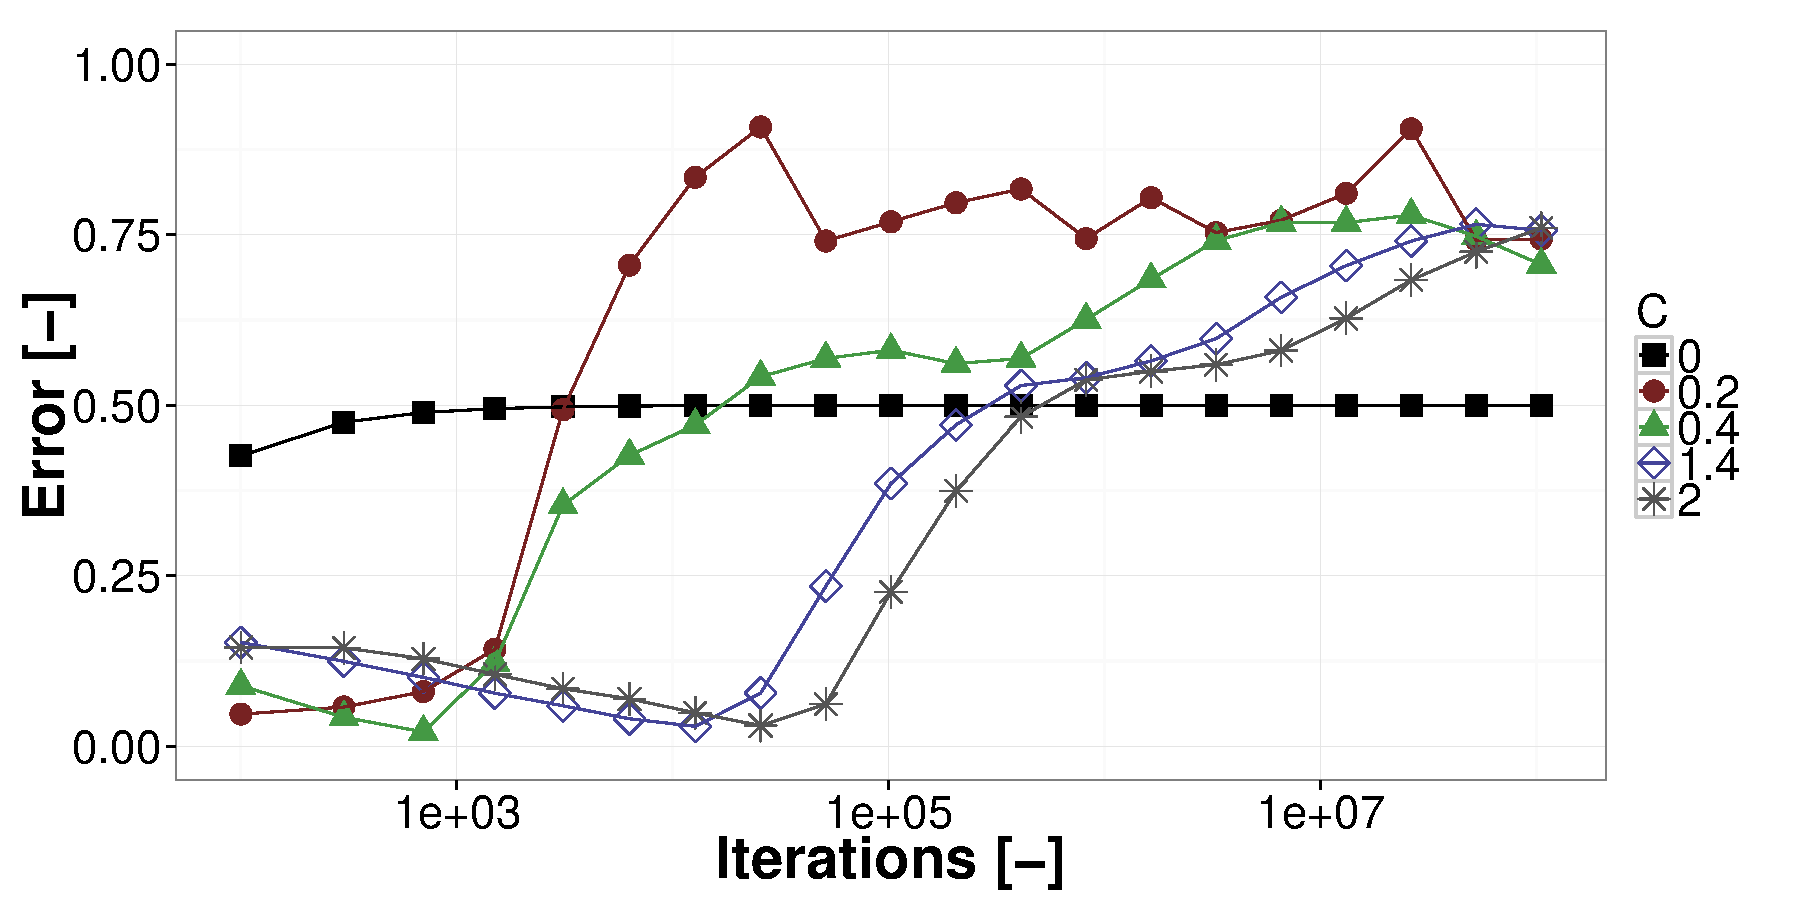
\includegraphics[width=0.8\textwidth]{figures/brps-MCTS-UCT.pdf} \\
{\small MCTS-UCT with stochastic tie-breaking} \\
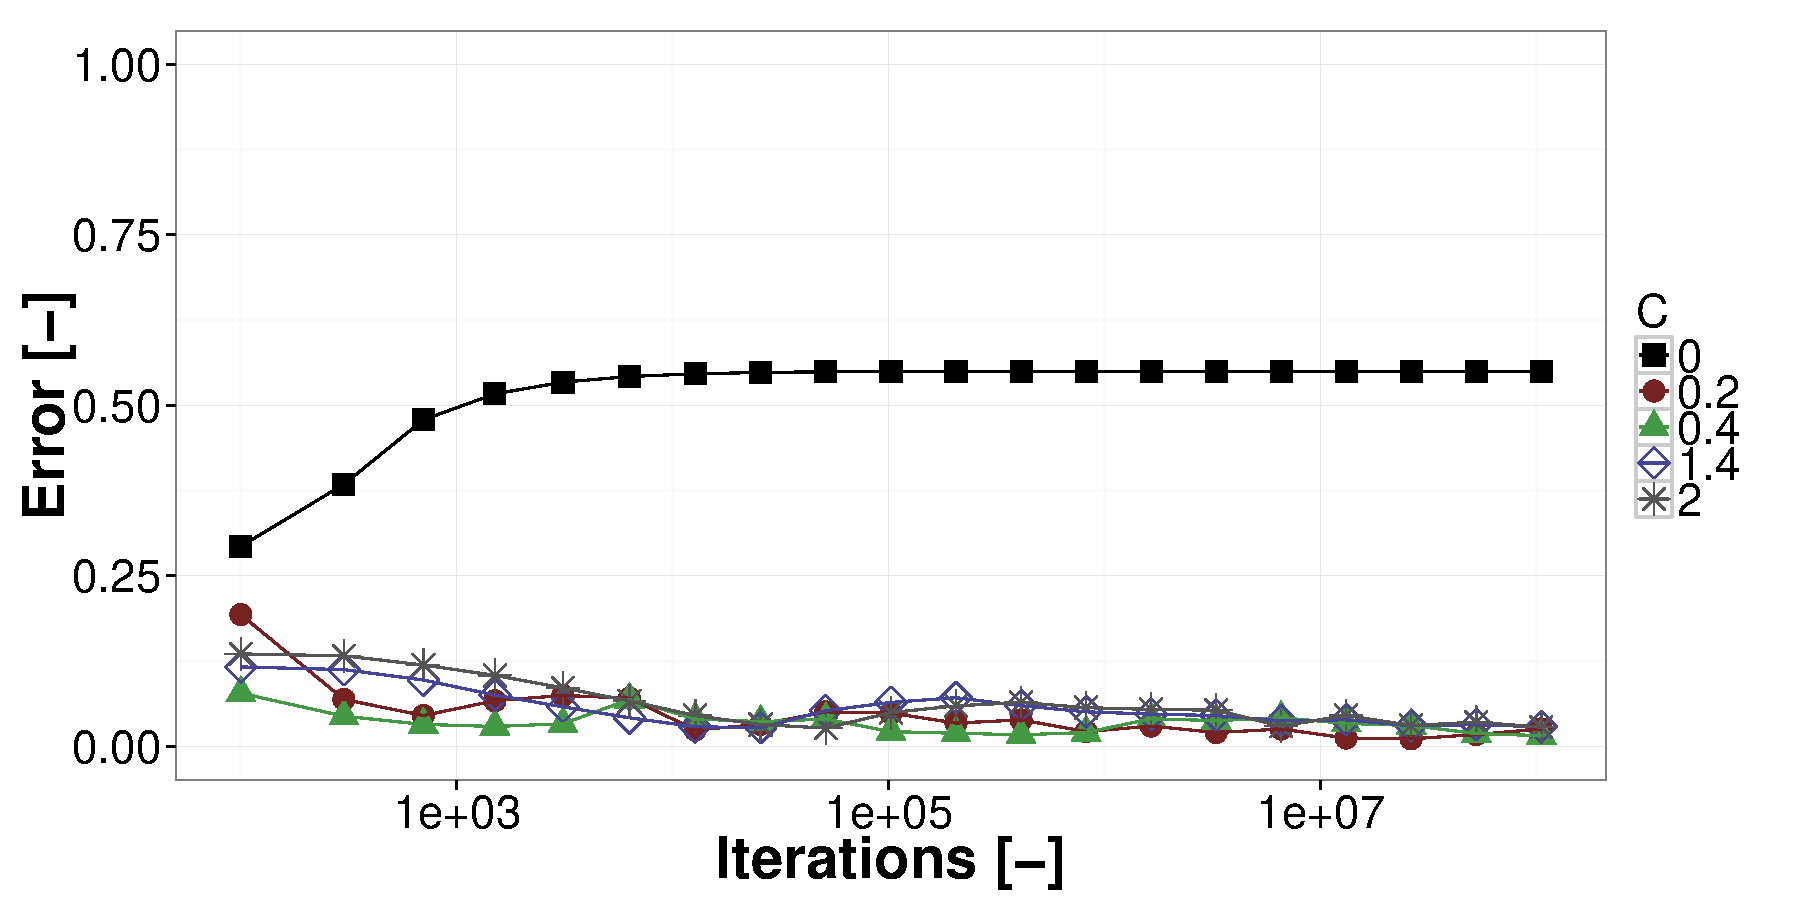
\includegraphics[width=0.8\textwidth]{figures/brps-MCTS-UCT-NONDET.pdf} \\
\end{tabular}
\caption{Exploitability of strategies of recommended by MCTS-UCT over time in Biased Rock, Paper, Scissors. Vertical axis represents exploitability. }
\label{fig:expl-brps1}
\end{figure}

\begin{figure}[t!]
\centering
\begin{tabular}{c}
%{\small MCTS-UCT (fully deterministic)} \\
%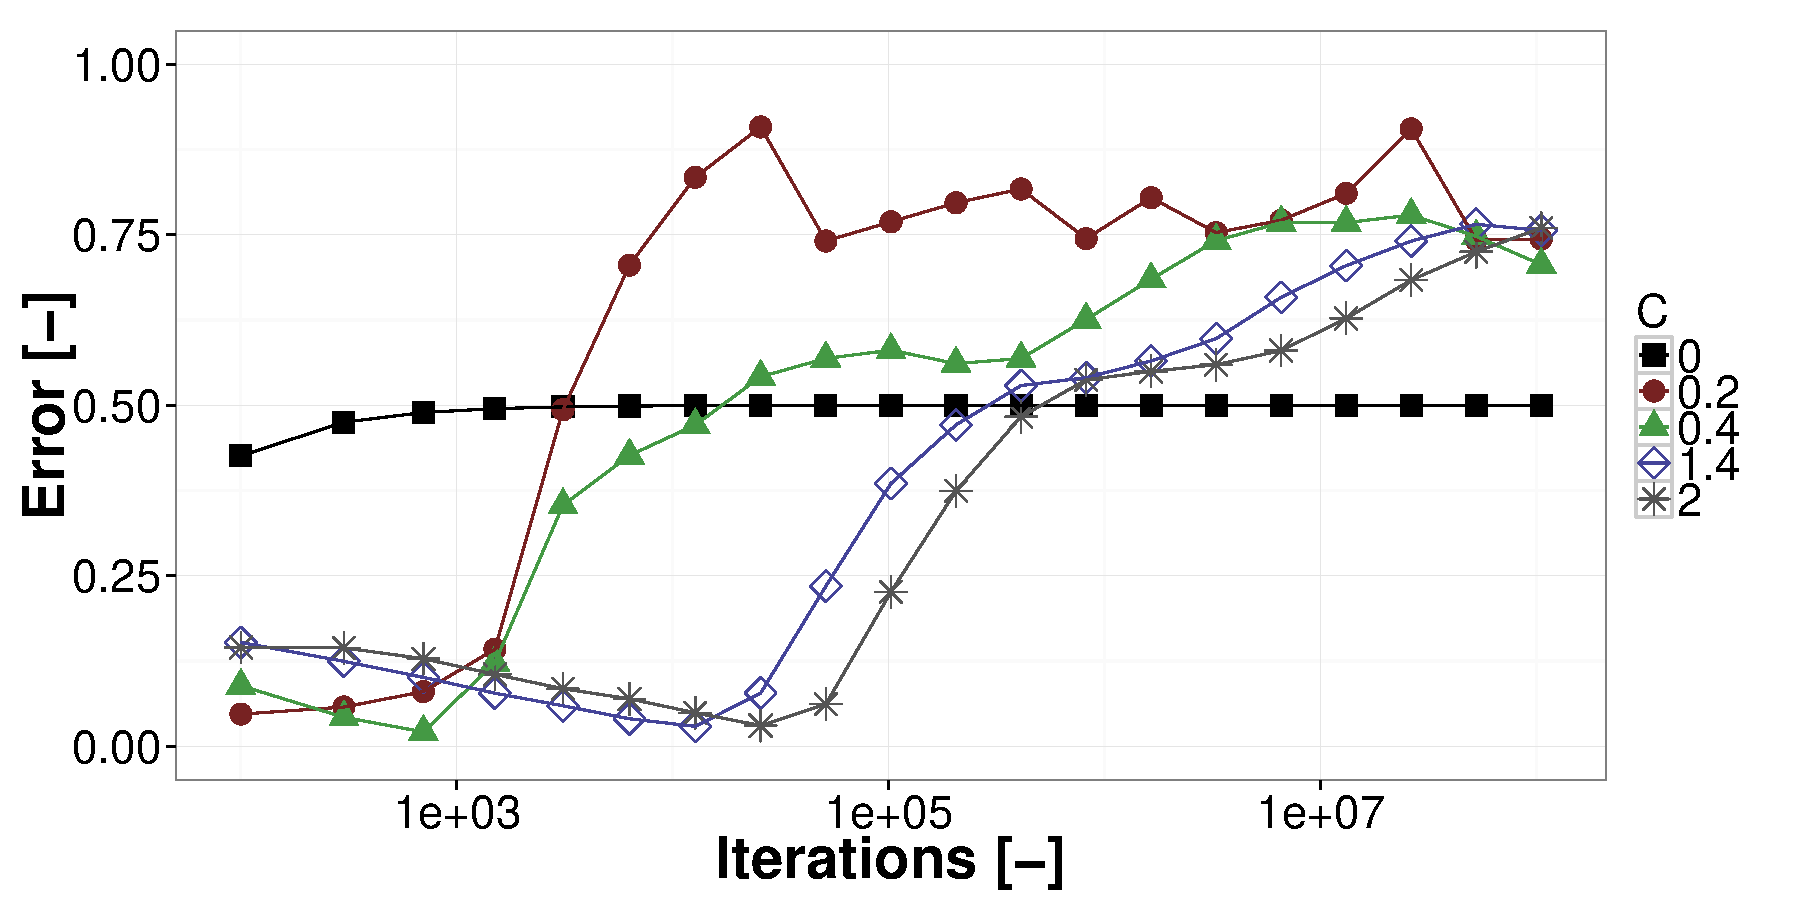
\includegraphics[width=0.4\textwidth]{figures/brps-MCTS-UCT.pdf} \\
%{\small MCTS-UCT with stochastic tie-breaking} \\
%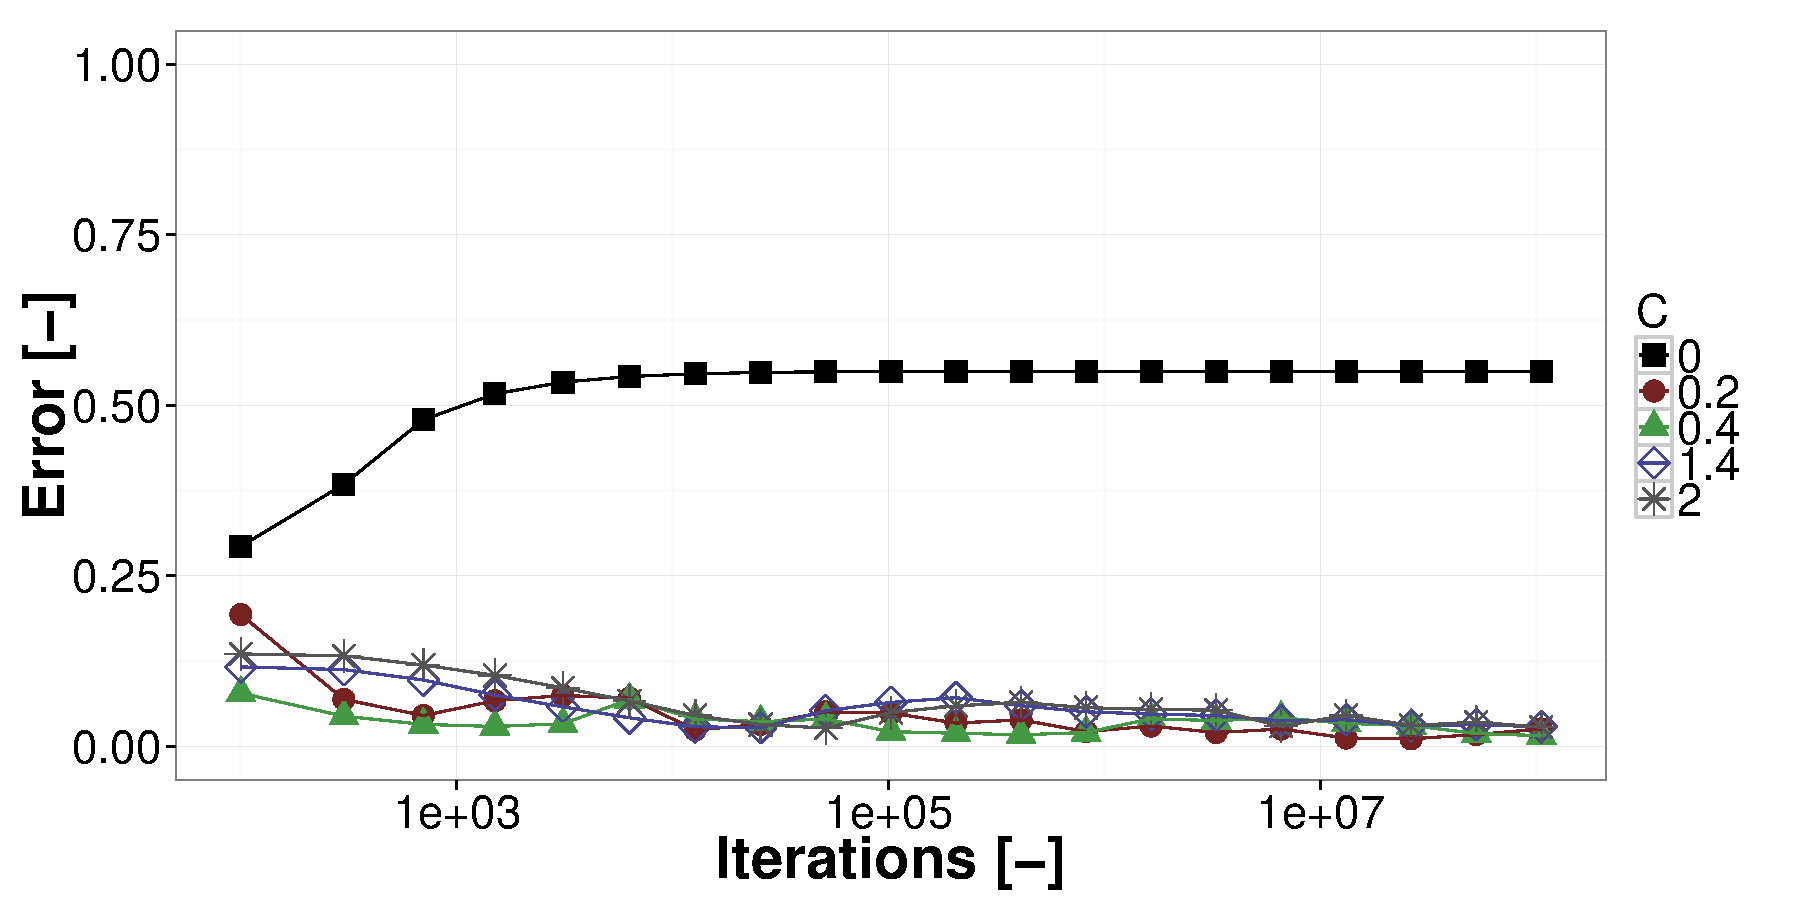
\includegraphics[width=0.4\textwidth]{figures/brps-MCTS-UCT-NONDET.pdf} \\
{\small MCTS-Exp3} \\
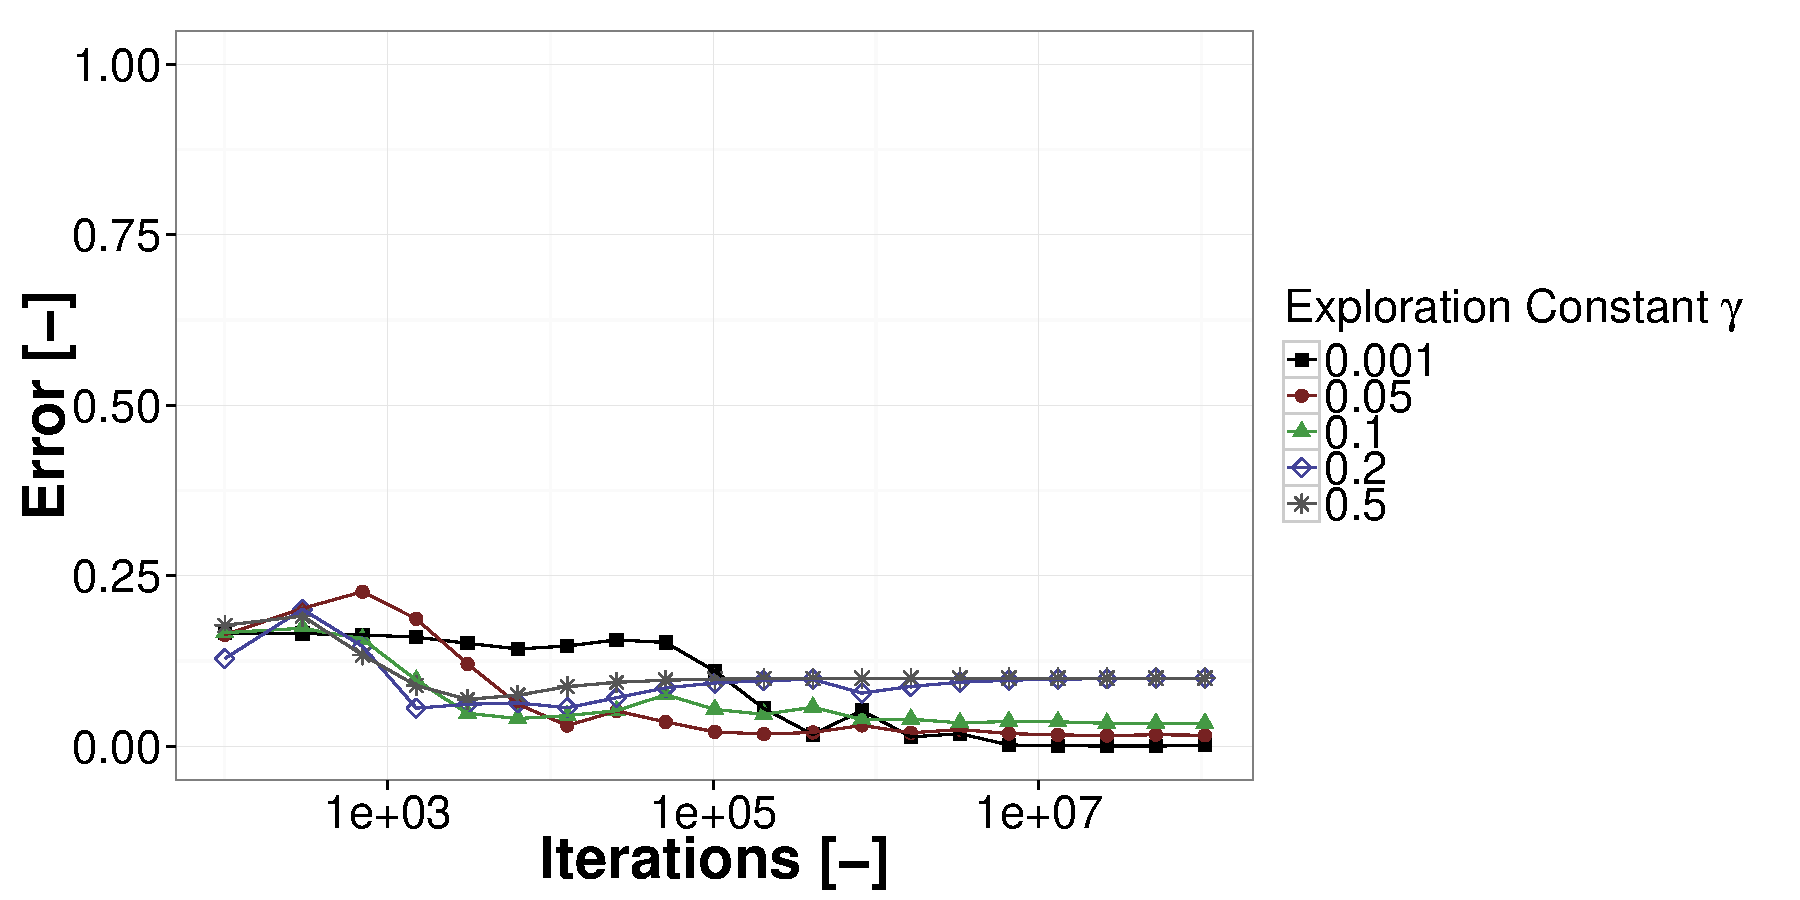
\includegraphics[width=0.8\textwidth]{figures/brps-MCTS-EXP3.pdf} \\
{\small MCTS-RM} \\
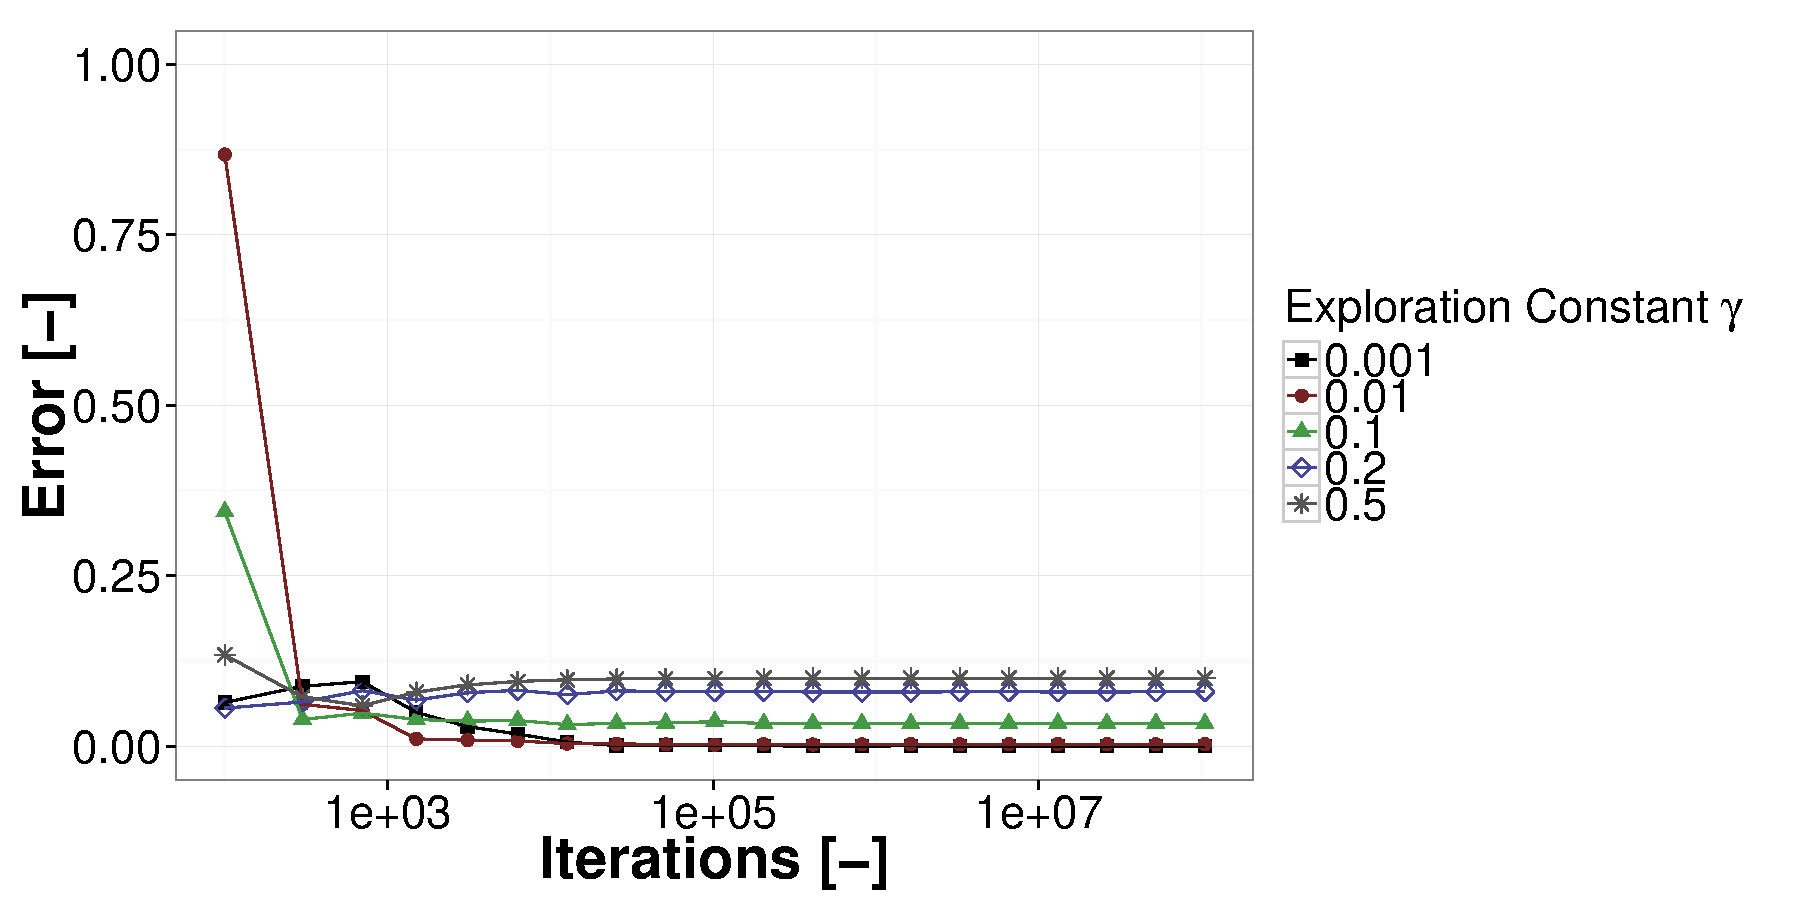
\includegraphics[width=0.8\textwidth]{figures/brps-MCTS-RM.pdf} \\
\end{tabular}
\caption{Exploitability of strategies of recommended by MCTS-Exp3 and MCTS-RM over time in Biased Rock, Paper, Scissors. Vertical axis represents exploitability. }
\label{fig:expl-brps2}
\end{figure}

We then tried adding a stochastic tie-breaking rule to the UCT selection mechanism typically used in MCTS implementations, which chooses an
action randomly when the scores of the best values are ``tied'' (less than $0.01$ apart).
Figure~\ref{fig:expl-brps1}, bottom figure shows the convergence.
One particularly striking observation is that this simple addition leads to a large drop in resulting exploitability, where exploitability
ranges from $[0.5,0.8]$ in the deterministic case, compared to $[0.01,0.05]$ with stochastic tie-breaking. Therefore, stochastic tie-breaking is
enabled in all of our experiments.

In summary, with this randomization UCT appears to be converging to an approximate equilibrium but not to an
exact equilibrium, which is similar to results of UCT in Kuhn poker~\cite{Ponsen11Computing}.

%mlanctot: is this true? %bbosansky: yes, we have run again experiments with randomized uct where deterministic uct had been used before

%\mlanctot{I noticed Vilo added his example to the SM-MCTS section so please modify this paragraph as necessary. Maybe it can be
%removed entirely?} We investigated this further and found a possible
%explanation of this behavior. Consider the matrix game on the right of Figure~\ref{fig:egMatrixGames} in Section~\ref{sec:smg}.
%Suppose DUCT is run on this game and players deterministically prefer the left-action.
%DUCT will always recieve rewards 0 and the exploration bias term will cause the players to round-robin over the actions indefinitely.
%However, each player can than improve by playing first action with probability 1. Breaking ties stochastically will lead the algorithm to
%discover the 1 and -1 rewards with high probability and allow the algorithm the break out or avoid this synchronization trap.

\subsection{Offline Equilibrium Computation} \label{sec:eval:offline}

We now compare the offline performance of the algorithm on all the remaining games.
We measure the overall computation time for each of the algorithms and number of evaluated nodes -- \ie nodes for which the main method of the backward induction algorithm executed (\ie nodes evaluated by serialized alpha-beta algorithms are not included in this count, since they may be evaluated repeatedly).
Unless otherwise stated, each data point represents a mean of at least $30$ runs.
% mlanctot: check this %bbosansky: ?

\subsubsection{Goofspiel}
\begin{figure}[t!]
\centering
	\begin{subfigure}{0.49\textwidth}
 		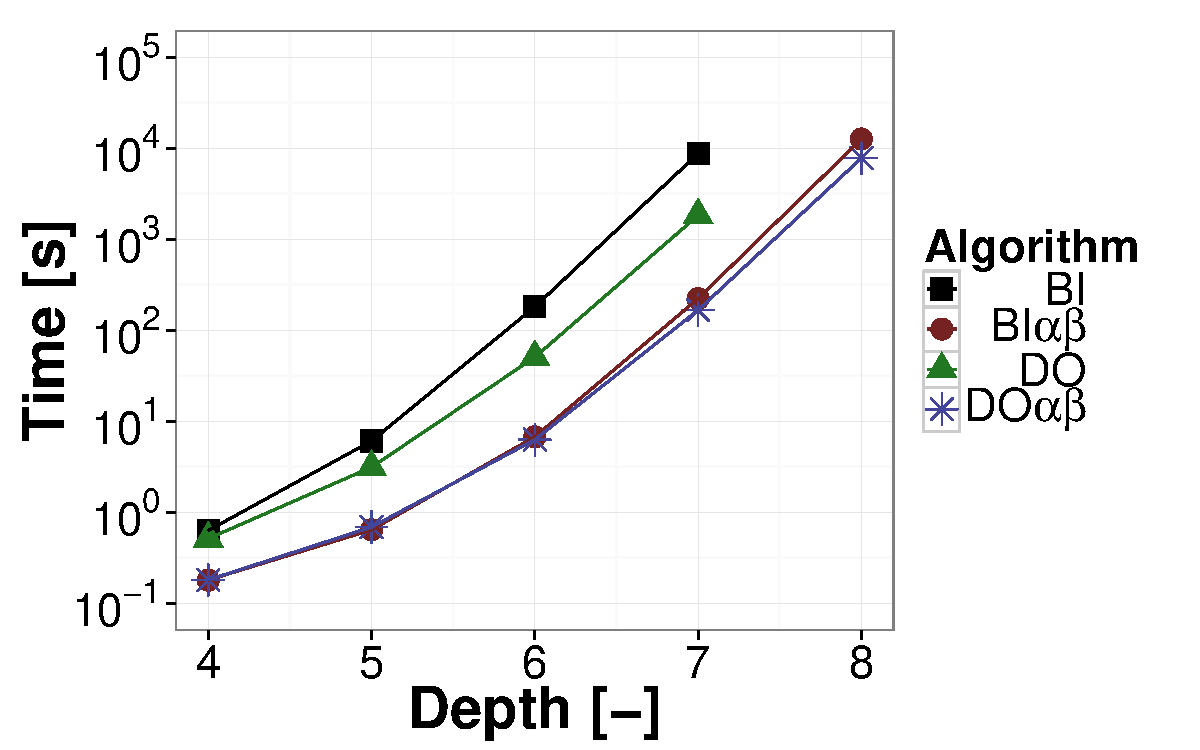
\includegraphics[width=1\textwidth]{figures/GS-BT-NF.pdf}\caption{}\label{fig:off:res:gs-bt}
 	\end{subfigure}
	\begin{subfigure}{0.49\textwidth}
 		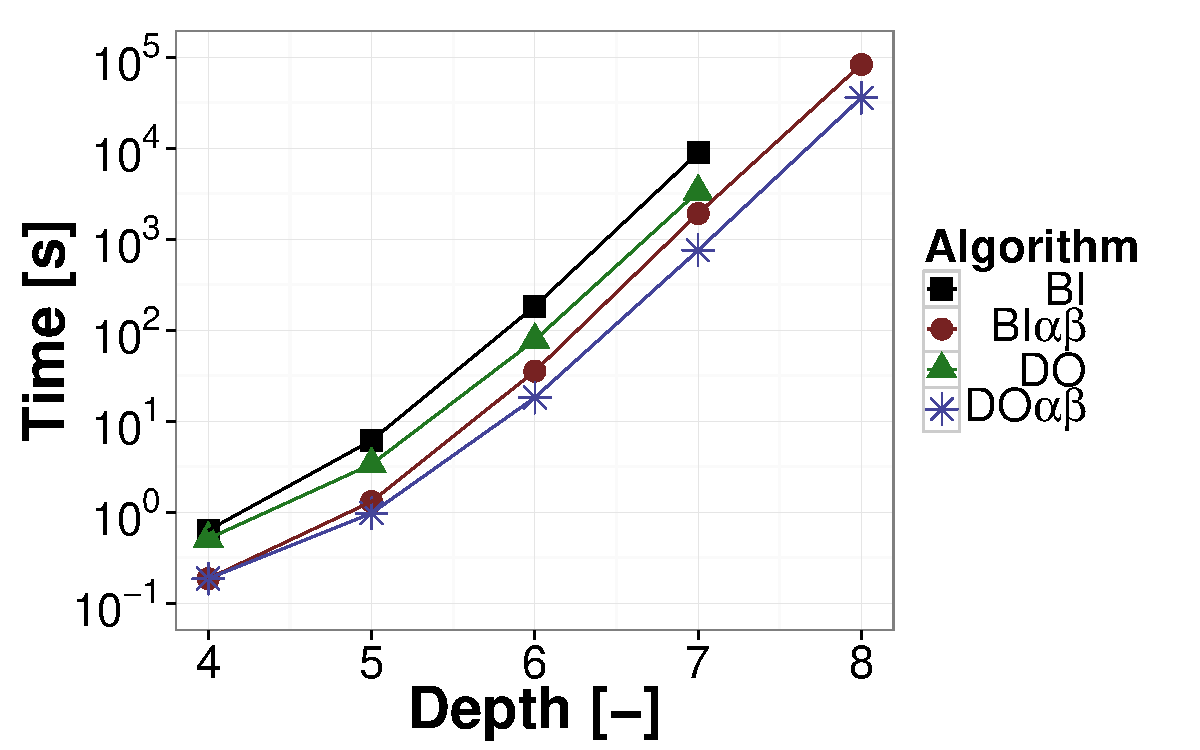
\includegraphics[width=1\textwidth]{figures/GS-BF-NF.pdf}\caption{}\label{fig:off:res:gs-bf}
 	\end{subfigure}
\caption{Running times of exact algorithms on Goofspiel with fixed sequence of cards for increasing size of the deck; subfigure (a) depicts the results with win-tie-lose utilities, (b) depicts the results with point utilities.} \label{fig:off:res:gs}
\end{figure}

We now describe the results for the card game Goofspiel.
First, we analyze the games with fixed sequences of the cards.

\paragraph{Exact algorithms with fixed sequences}
The results are depicted in Figure~\ref{fig:off:res:gs} (note the logarithmic vertical scale), where the left subfigure depicts the results for win-tie-lose utilities and the right subfigure depicts the results for point utilities.
\reviewchange{We present the mean results from 10 different fixed sequences.}
The comparison on the win-tie-lose variant shows that there is a significant number of subgames with pure Nash equilibrium that can be computed using serialized alpha-beta algorithms.
Therefore, the performance of $\biab$ and $\doab$ is fairly similar and the gap only slowly increases in favor of $\doab$ with the increasing size of the game.
Since serialized alpha-beta is able to solve a large portion of subgames, both of these algorithms significantly reduce the number of the states visited by the backward induction algorithm.
While \textsc{BI} algorithm evaluates than $3.2\times10^7$ nodes in the setting with $7$ cards in more than $2.5$ hours, $\biab$ evaluates only $198,986$ nodes in less than $4$ minutes.
The performance is further improved by $\doab$ that evaluates on average $79,105$ nodes in less than $3$ minutes.
The overheads are slightly higher in case of $\doab$; hence, the time difference between $\doab$ and $\biab$ is relatively small compared to the difference in evaluated nodes.
Finally, the results show that even simple \textsc{DO} algorithm without serialized alpha-beta search can improve the performance of \textsc{BI}.
In the setting with $7$ cards, \textsc{DO} evaluates more than $6\times10^6$ nodes which takes on average almost 30 minutes.

\reviewchange{The results for the point utilities are the same for BI, while DO is slightly worse.
On the other hand, the success of serialized alpha-beta algorithm is significantly lower and it takes both algorithms much more time to solve games of same size.
With $7$ cards, $\biab$ now evaluates more than $2\times10^6$ nodes and it takes the algorithm on average $32$ minutes to find the solution.
$\doab$ is still the fastest and it evaluates more than $3\times10^5$ nodes in less than $13$ minutes on average.}

The performance of algorithms $\biab$ and $\doab$ represent a significant improvement over the results of the pruning algorithm
SMAB presented in \cite{Saffidine12SMAB}.
In their work, the number of evaluated nodes was at best around $29\%$, and the running time improvement was only marginal.

\reviewchange{
\paragraph{Exact algorithms with a stochastic sequence}

\begin{figure}[t!]
\centering
	\begin{subfigure}{0.49\textwidth}
 		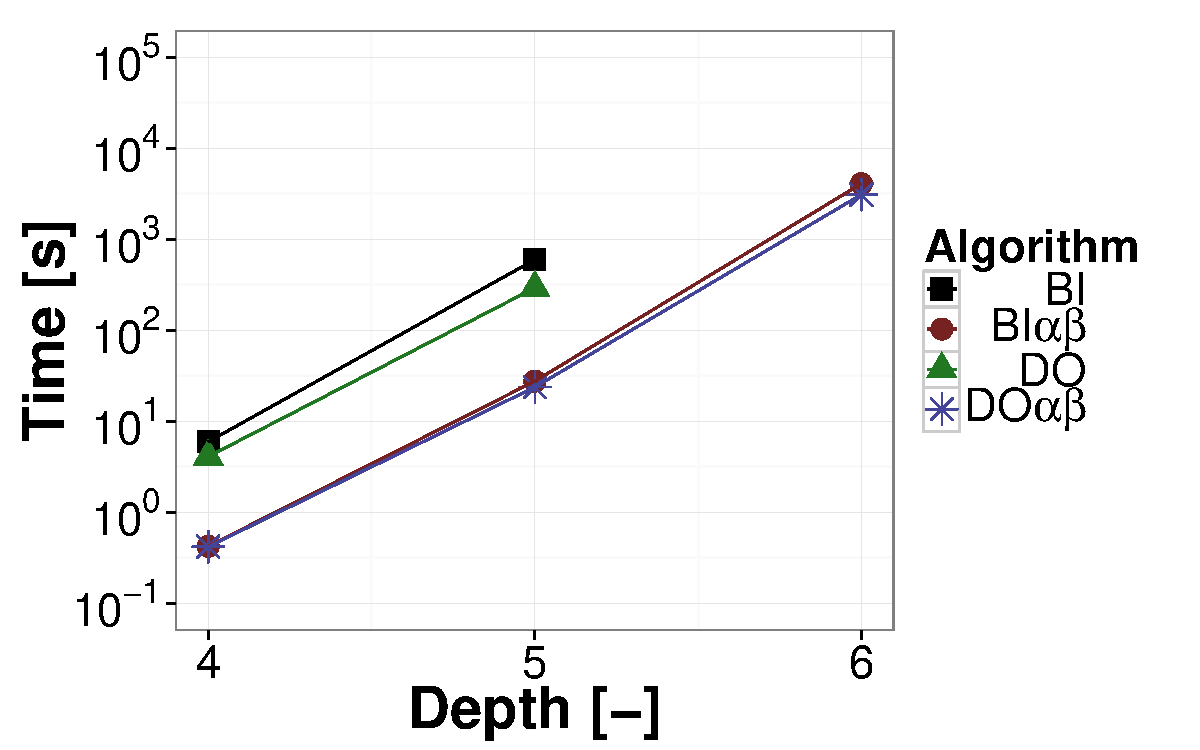
\includegraphics[width=1\textwidth]{figures/GS-BT-NN.pdf}\caption{}\label{fig:off:res:gsn-bt}
 	\end{subfigure}
	\begin{subfigure}{0.49\textwidth}
 		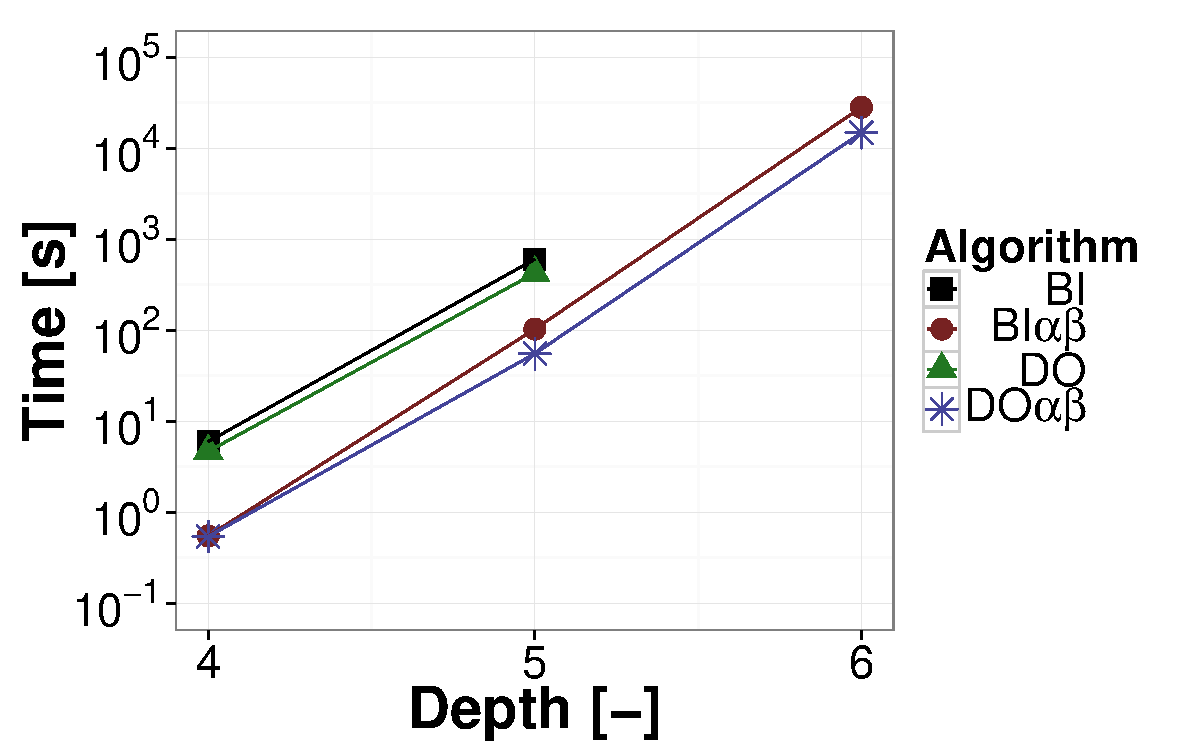
\includegraphics[width=1\textwidth]{figures/GS-BF-NN.pdf}\caption{}\label{fig:off:res:gsn-bf}
 	\end{subfigure}
\caption{Running times of exact algorithms on Goofspiel with chance nodes for increasing size of the deck; subfigure (a) depicts the results with win-tie-lose utilities, (b) depicts the results with point utilities.} \label{fig:off:res:gsn}
\end{figure}

Next we compare the exact algorithms in the variant of Goofspiel with standard chance nodes.
Introducing another branching due to moves by chance causes a significant increase in the size of the game tree.
For $7$ cards, the game tree has more than $10^{11}$ nodes, which is $4$ orders of magnitude more than in the case with fixed sequence of cards.
The results depicted in Figure~\ref{fig:off:res:gsn} show that the games become quickly too large to solve exactly and the fastest algorithms solved games with at most $6$ cards.
Relative performance of the algorithms, however, is similar to the case with fixed sequence.
With win-tie-lose utilities, serialized alpha-beta is again able to find pure NE in most of the subgames and prunes out a large fraction of the states.
For the game with $5$ cards, BI evaluates more than $2 \times 10^6$ nodes in almost $10$ minutes, while $\biab$ evaluates only $17,315$ nodes in $27$ seconds and $\doab$ evaluates $6,980$ nodes in $23$ seconds.
As before, serialized alpha-beta algorithm is less helpful in the case with point utilities.
Again with $5$ cards, $\biab$ evaluates $91,419$ nodes in more than $100$ seconds and $\doab$ evaluates $14,536$ nodes in almost $55$ seconds.
}

\paragraph{Sampling algorithms with fixed sequences}

\begin{figure}[t!]
	\begin{subfigure}{1\textwidth}
		\centering
		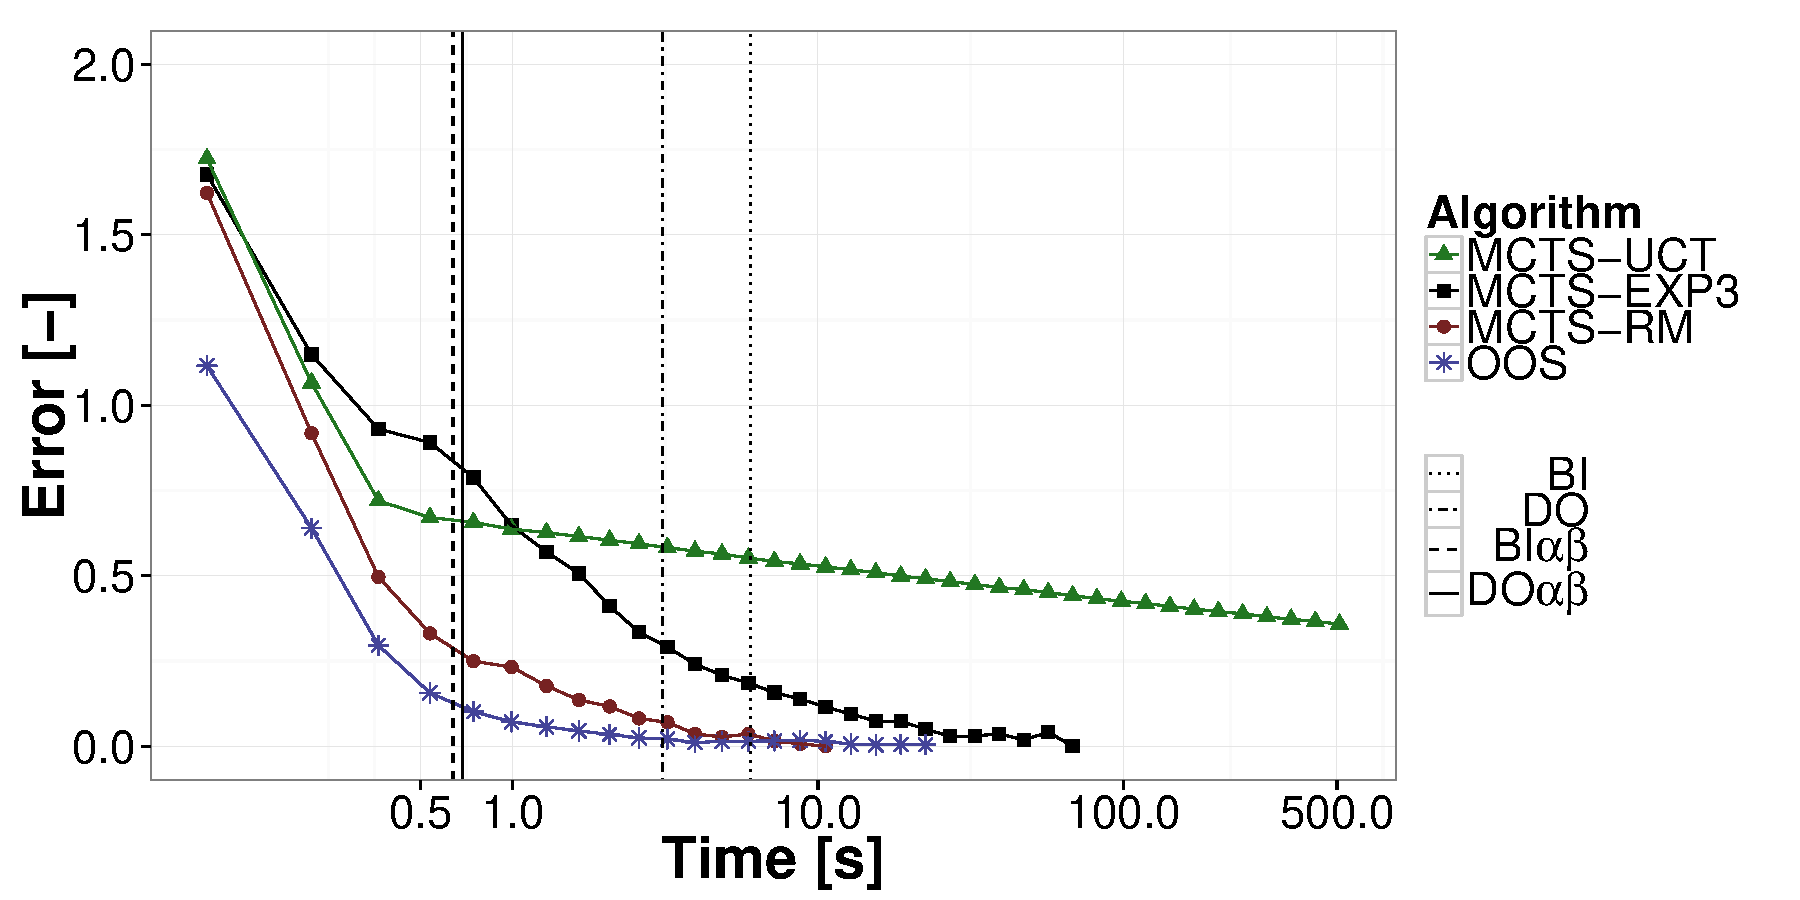
\includegraphics[width=0.85\textwidth]{figures/convergence-gs-tf.pdf}%\caption{}\label{fig:off:conv:gs-bt}
	\end{subfigure}
	\begin{subfigure}{1\textwidth}
		\centering
		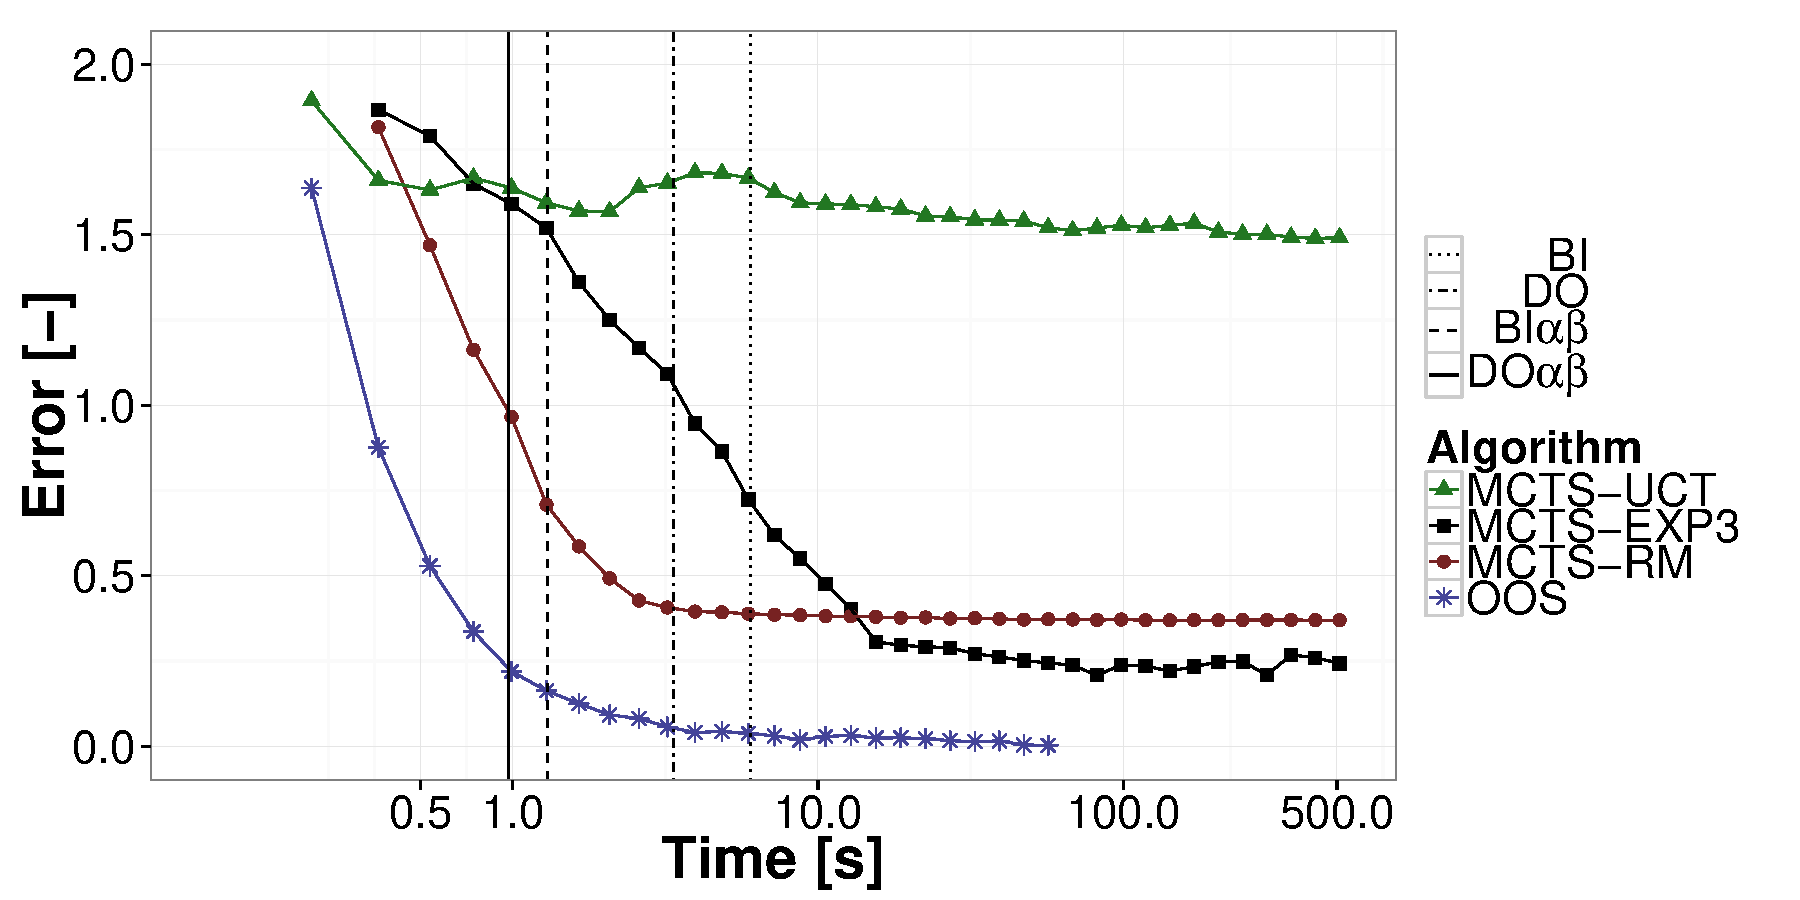
\includegraphics[width=0.85\textwidth]{figures/convergence-gs-ff.pdf}%\caption{}\label{fig:off:conv:gs-bf}
	\end{subfigure}
\caption{Convergence of sampling algorithms on Goofspiel with $5$ cards and fixed sequence of cards.
Vertical lines correspond to computation times for exact algorithms.
(Top) Goofspiel with win-tie-lose utility values;
(Bottom) Goofspiel with point utilities.} \label{fig:off:conv:gs}
\end{figure}

We now turn to the analysis of the convergence of the sampling algorithms -- \ie their ability to approximate Nash equilibrium strategies of the complete game.
Figure~\ref{fig:off:conv:gs} depicts the results for Goofspiel game with $5$ cards with fixed sequence of cards (note the logarithmic horizontal scale).
We compare MCTS algorithms with three different selection functions (UCT, Exp3, and RM), and OOS.
The results are means out of $30$ runs of each algorithm.
Due to the different selection and update functions, the algorithms differ in the number of iterations per second.
RM is the fastest with more than $2.6\times 10^5$ iterations per second, OOS has around $2\times10^5$ iterations, UCT $1.9\times10^5$, and Exp3 only $5.4\times10^4$ iterations.

The results show that OOS converges the fastest out of all sampling algorithms.
This is especially noticeable in the point-utility settings, where none of the other sampling algorithms were approaching zero error due to the exploration.
MCTS with RM selection function is only slightly slower in the win-tie-lose case, however, other two selection functions perform worse.
While Exp3 eventually converges close to $0$ in the win-tie-lose case, the exploitability of UCT decreases rather slowly and it was still over $0.35$ at the time limit of $500$ seconds.
The best $C$ constant for UCT was 5 in win-tie-lose setting, and $10$ in the point utility setting.
While setting lower constant typically improved slightly the
convergence during the first iterations, the final error was always larger.
%Moreover, when we have not used randomization in UCT, the algorithm was not able to converge to error lower than $0.5$ in the time limit.
%On the other hand, both OOS and RM confirm their quick convergence, witch is aligned with previous results~\cite{Lanctot13Goofspiel}.
The vertical lines represent times for exact algorithms.
In the win-tie-lose case, $\biab$ is slightly faster and finishes first in $0.64$ second, followed by $\doab$ ($0.69$ seconds), \textsc{DO} ($3.1$ seconds), and \textsc{BI} ($6$ seconds).
In the point case, $\doab$ is the fastest ($0.97$ seconds), followed by $\biab$ ($1.3$ seconds), followed by \textsc{DO} and \textsc{BI} with similar times as in the previous case.

\reviewchange{
\paragraph{Sampling algorithms with a stochastic sequence}

\begin{figure}[t!]
	\begin{subfigure}{1\textwidth}
		\centering
		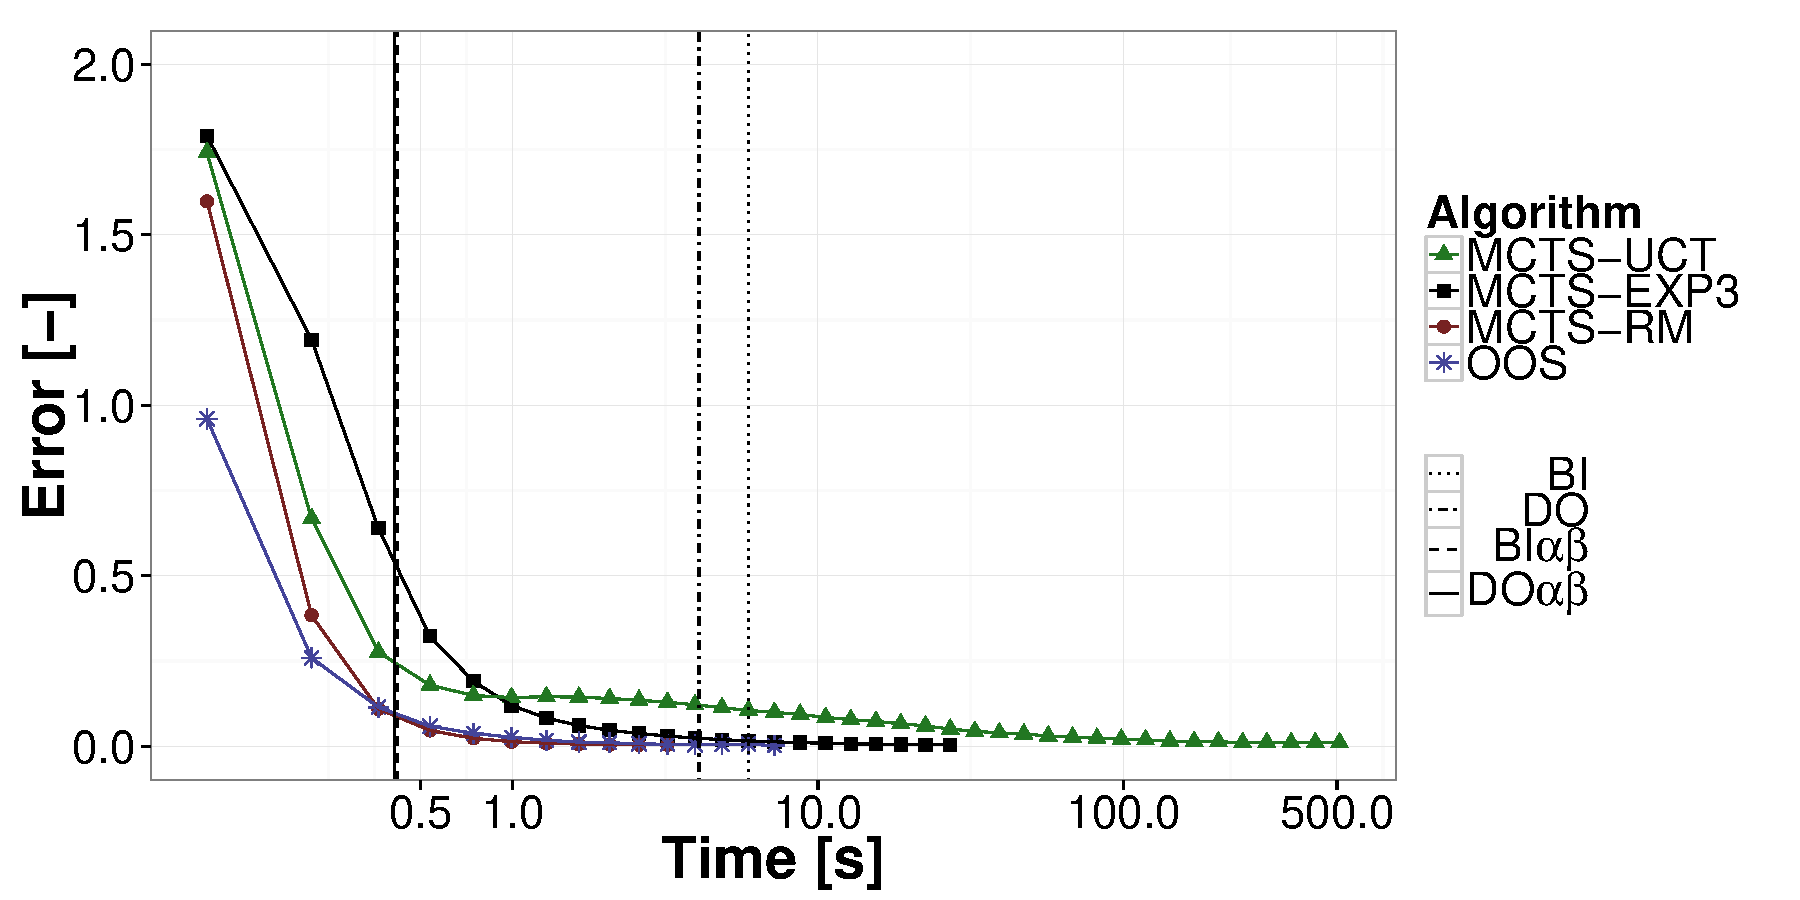
\includegraphics[width=0.85\textwidth]{figures/convergence-gs-tn.pdf}%\caption{}\label{fig:off:conv:gs-bt}
	\end{subfigure}
	\begin{subfigure}{1\textwidth}
		\centering
		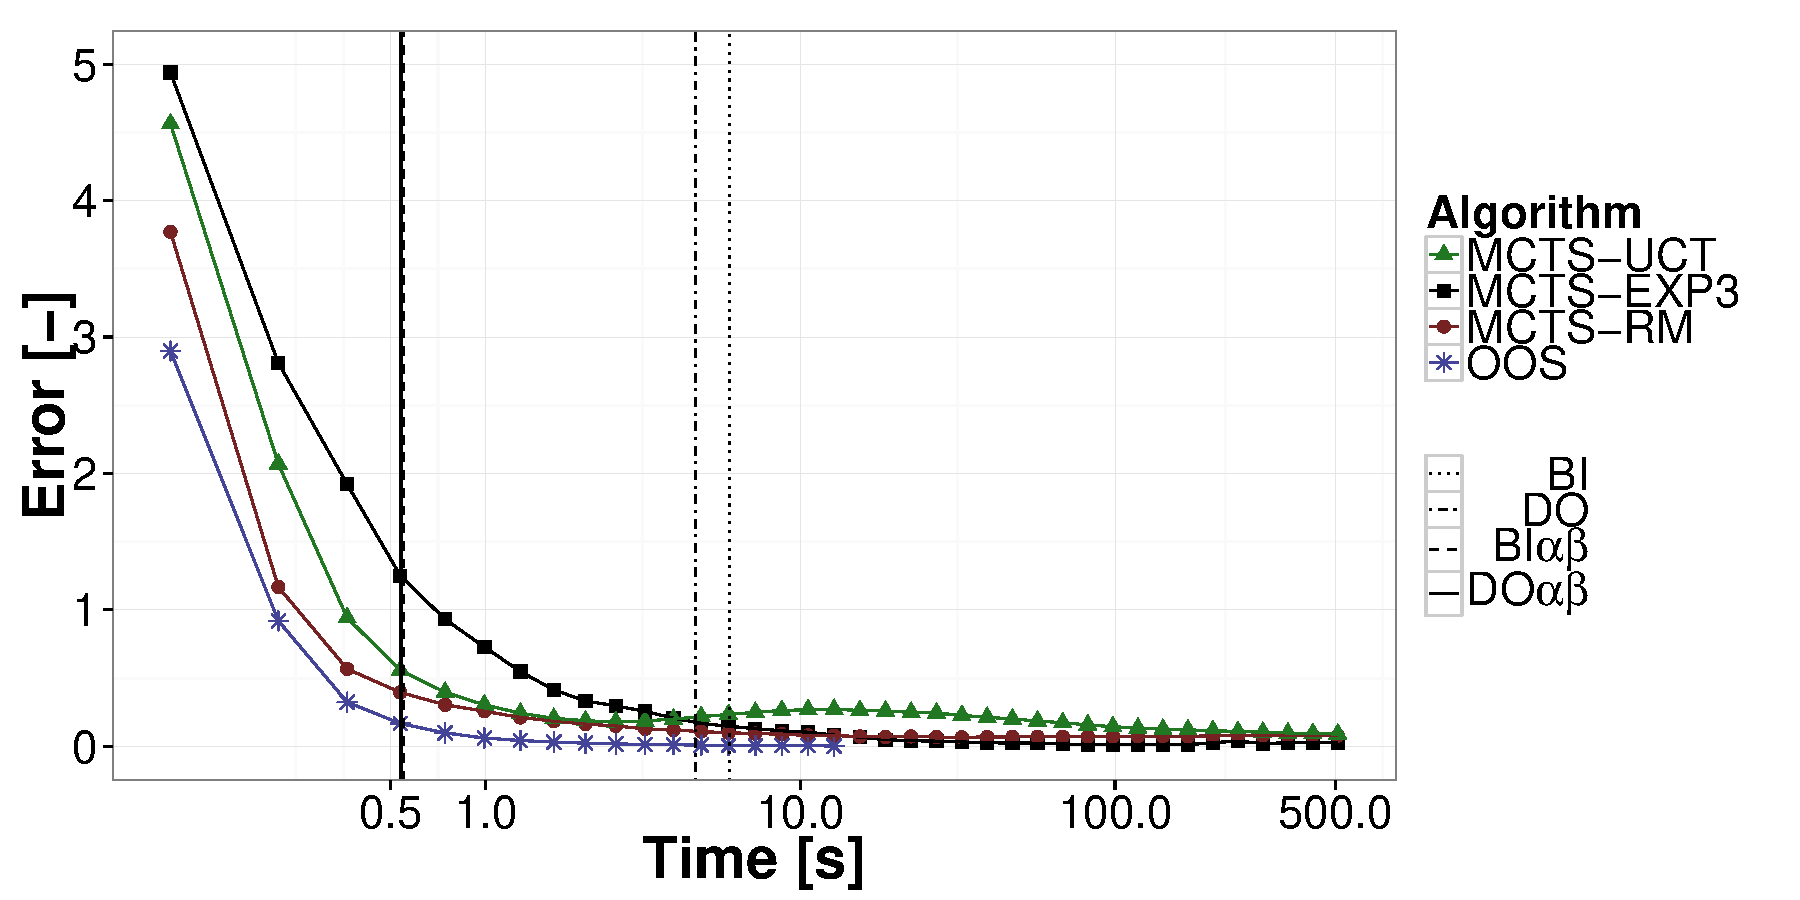
\includegraphics[width=0.85\textwidth]{figures/convergence-gs-fn.pdf}%\caption{}\label{fig:off:conv:gs-bf}
	\end{subfigure}
\caption{Convergence of sampling algorithms on Goofspiel with $4$ cards and chance nodes.
Vertical lines correspond to computation times of exact algorithms.
(Top) Goofspiel with win-tie-lose utility values;
(Bottom) Goofspiel with point utilities.} \label{fig:off:conv:gsn}
\end{figure}

We also performed the experiments in the setting with chance nodes.
Due to the size of the game tree, we have reduced the number of cards to $4$, since the size of this game tree is comparable to the case with $5$ cards and fixed sequence of cards.
The results depicted in Figure~\ref{fig:off:conv:gsn} show a similar behavior of the sampling algorithms as we have observed in the previous case.
OOS converges the fastest, followed by RM, and EXP3.
Main difference is in the convergence of UCT, however, this is mostly due to the fact that pure NE exists in Goofspiel with 4 cards; hence, UCT can better identify the best action to play and converges more quickly to less exploitable strategy than in the case with 5 cards.
Surprisingly, the convergence of the algorithms does not change that dramatically with the introduction of point utilities as in the previous case.
The main reason is that the range of the utility values is smaller compared to the previous case (there is one card less in the present setting and the missing cards has the highest value).
For comparison, we again use the vertical lines to denote times of exact algorithms.
$\biab$ and $\doab$ are almost identically fast, with $\doab$ being slightly faster, followed by \textsc{DO} and \textsc{BI}.
}

\subsubsection{Pursuit-Evasion Games}
\begin{figure}
\centering
	\begin{subfigure}{0.49\textwidth}
		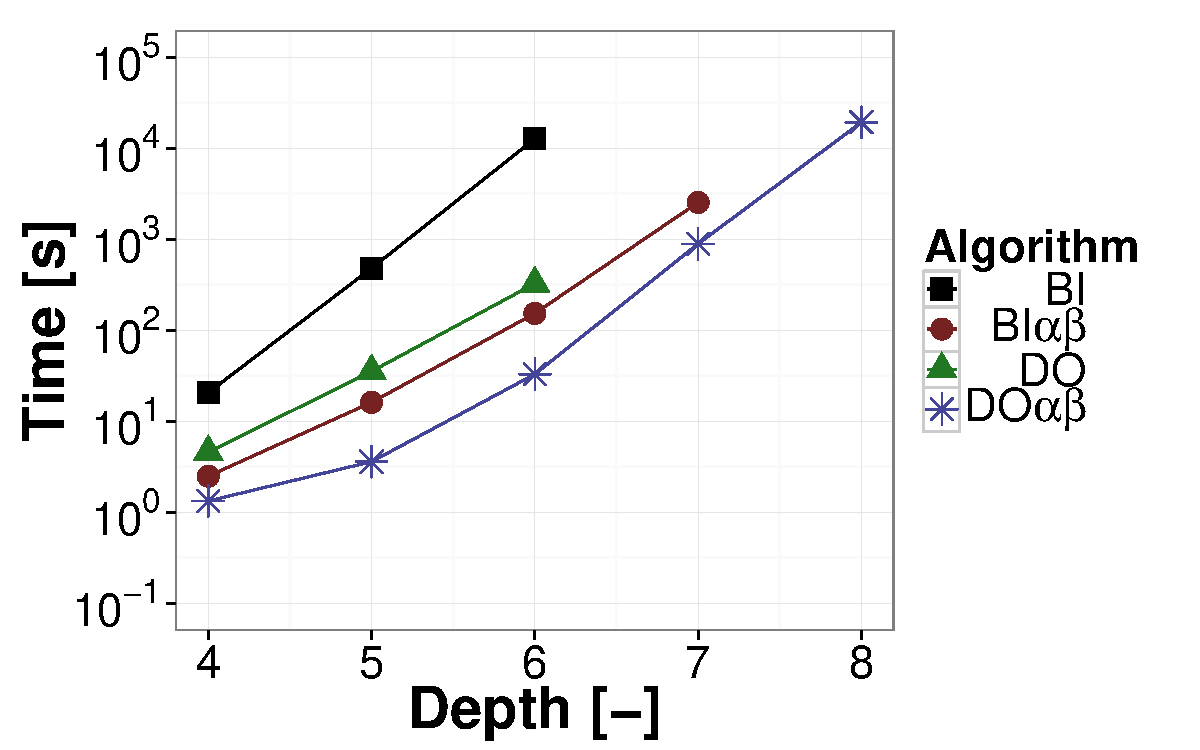
\includegraphics[width=1\textwidth]{figures/PEG4x4.pdf}\caption{}\label{fig:off:res:peg4}
	\end{subfigure}
	\begin{subfigure}{0.49\textwidth}
		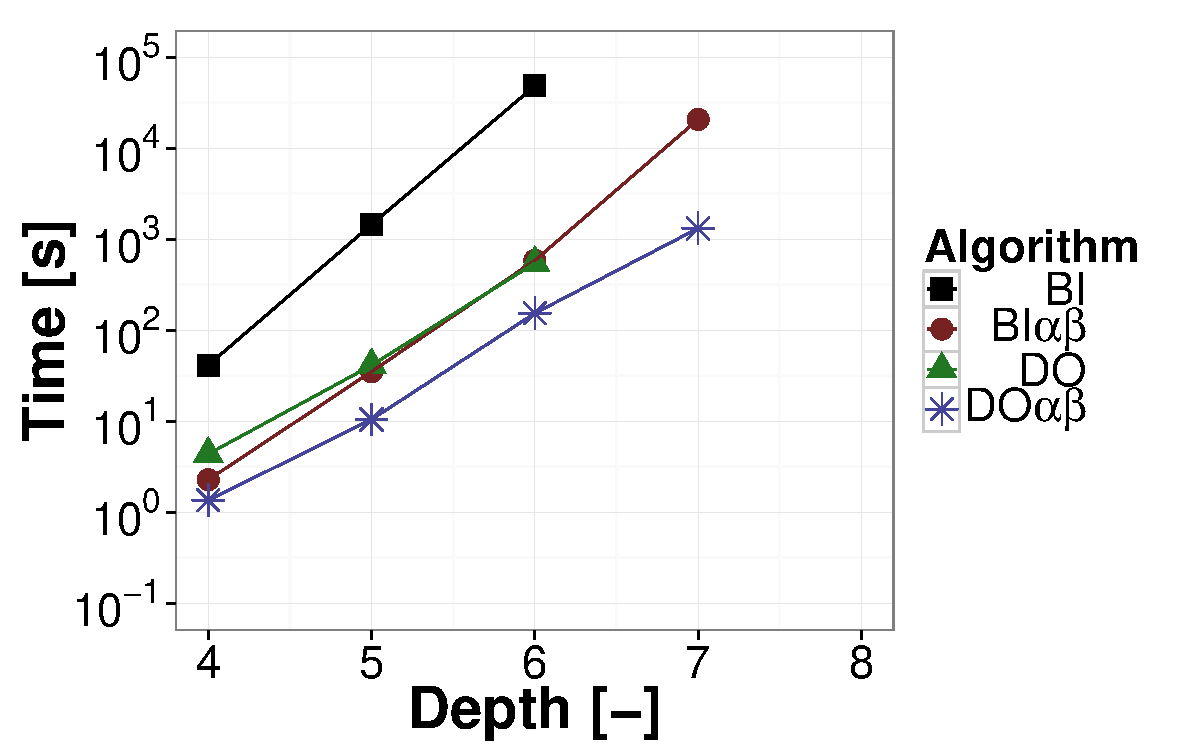
\includegraphics[width=1\textwidth]{figures/PEG5x5.pdf}\caption{}\label{fig:off:res:peg5}
	\end{subfigure}
\caption{Running times of exact algorithms on pursuit-evasion game with increasing number of moves: subfigure (a) depicts the results on $4\times4$ grid graph, (b) depicts results for $5\times5$ grid.} \label{fig:off:res:peg}
\end{figure}

The results on pursuit-evasion games show more significant improvement when comparing $\doab$ and $\biab$ (see Figure~\ref{fig:off:res:peg}). In all settings, the $\doab$ is significantly the fastest. When we compare the performance on graph $5\times5$ with depth set to $6$, \textsc{BI} evaluates more than $4.9\times10^7$ nodes that takes more than $13$ hours. On the other hand, $\biab$ evaluates on average $42001$ nodes taking almost $10$ minutes ($584$ seconds). Interestingly, the benefits of pure integration with alpha-beta search is not that helpful in this game.
This is apparent from results of \textsc{DO} algorithm that evaluates less than $2\times10^6$ nodes but it takes slightly over $9$ minutes on average ($547$ seconds). Finally, $\doab$ evaluates only $6692$ nodes and it takes the algorithm less than $3$ minutes.

Large parts of these pursuit-evasion games can be solved by serialized alpha-beta algorithms.
These parts typically corresponds to clearly winning, or clearly losing positions for a player; hence, serialized alpha-beta algorithms are able to prune substantial portion of the space.
However, since there are only two pursuit units, it is still necessary to use mixed strategies for final coordination (capturing the evader close to edge of the graph), and thus mixing strategy occurs near the end of the game tree.
Therefore, serialized alpha-beta is not able to solve all subgames, while double-oracle provides additional pruning since many of the actions in the subgames are leading to the same outcome and not all of them are required to find equilibrium strategies.
This causes additional improvement in computation time for $\doab$ compared to $\biab$ and all the other algorithms.%\vlisy{This argument is not very consistent with $\biab$ evaluating $\tfrac{1}{1000}$ of the nodes BI evaluates, while DO evaluating $\tfrac{1}{20}$. The reason is likely the cost of serialized searches.}

\begin{figure}[t!]
\centering
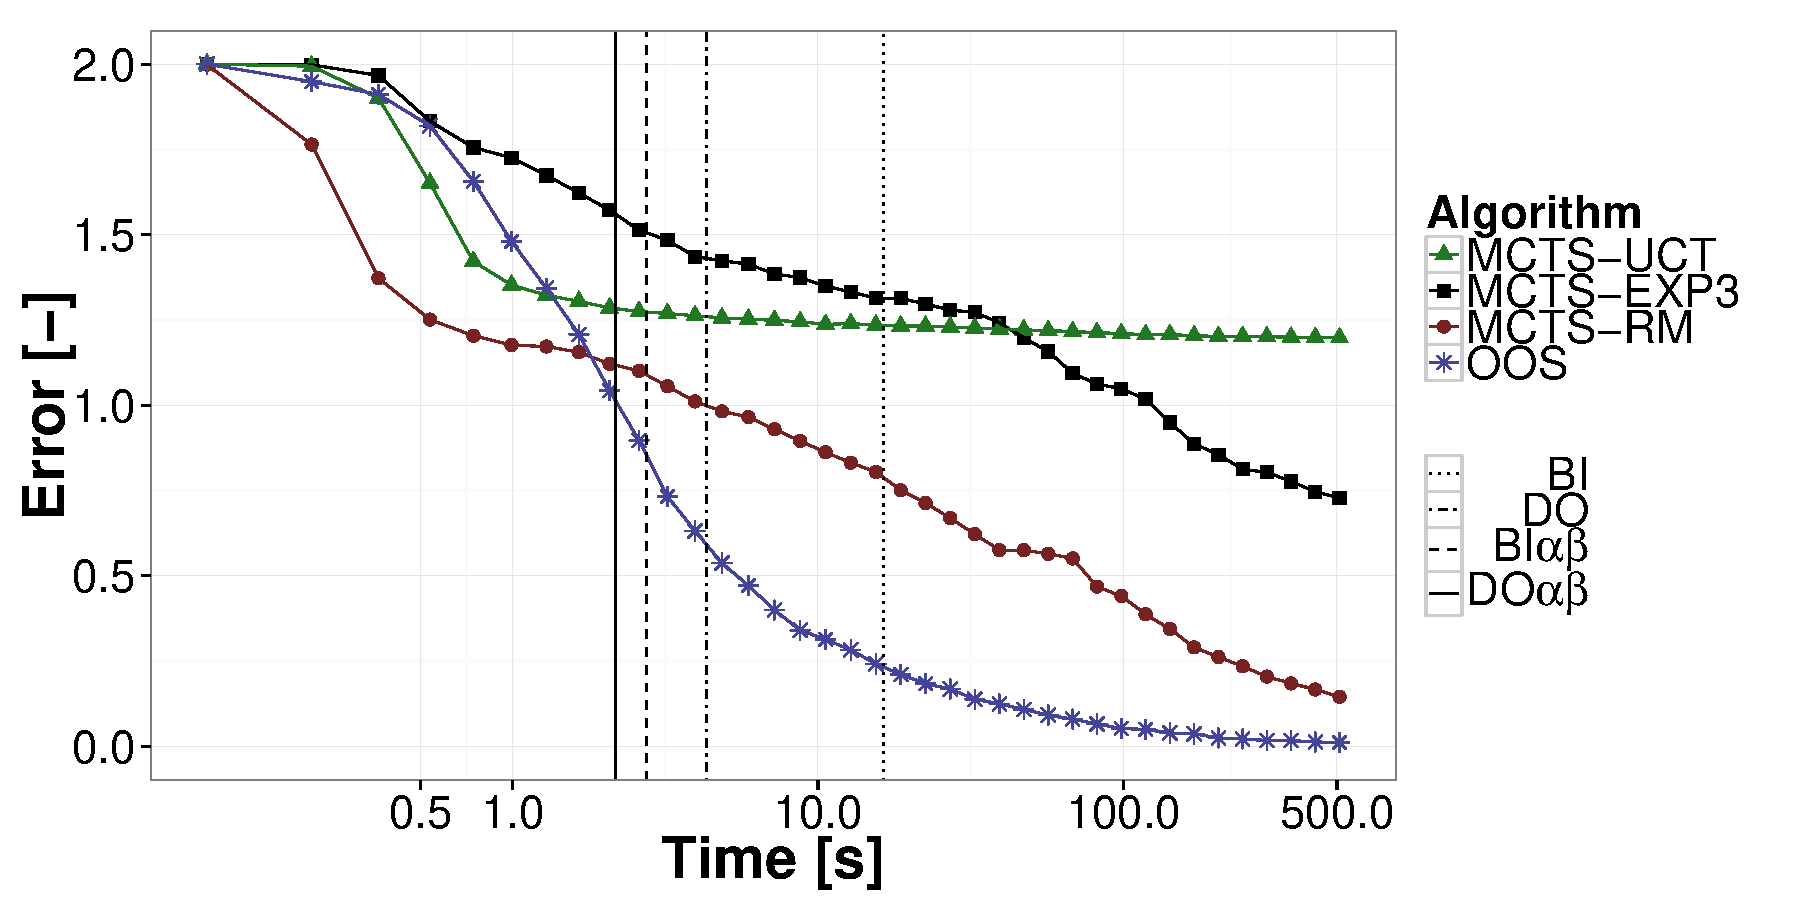
\includegraphics[width=0.85\textwidth]{figures/convergence-peg.pdf}
\caption{Convergence of sampling algorithms on pursuit-evasion game, on $4\times4$ graph, with depth set to $4$. The vertical lines correspond to computation times of exact algorithms.} \label{fig:off:conv:peg}
\end{figure}

We turn to convergence of the sampling algorithms.
In terms of number of iterations per second, again RM was the fastest and OOS the second fastest with similar performance as in Goofspiel.
UCT achieved slightly less ($1.7\times10^5$ iterations per second), and Exp3 only $2.6\times10^4$ iterations.
The results are depicted in Figure~\ref{fig:off:conv:peg} for the smaller $4\times4$ graph and $4$ moves for each player (note again the logarithmic horizontal scale).
The starting positions were selected such that there does not exist a pure NE strategy in the game.
The results again show that OOS is overall the fastest out of all sampling algorithms.
During the first iterations, RM preform similarly, however, OOS is able to keep the convergence rate, RM converges more slowly.
UCT again converges to an exploitable strategy with error $1.16$ at best in the time limit of $500$ seconds ($C=2$).
Finally, Exp3 is converging even more slowly than in Goofspiel.
The main difference between the games is the size of the branching factor for the second player (pursuer controls two simultaneously moving units), which can cause more difficulties for the sampling algorithms to estimate good strategies.

As before, the vertical lines represent times for exact algorithms.
In pursuit-evasion game of this setting, $\doab$ is slightly faster and finishes first in $2.77$ seconds, following by $\biab$ ($2.89$ seconds), \textsc{DO} ($5.48$ seconds), and \textsc{BI} ($12.5$).

\subsubsection{Oshi-Zumo}
\begin{figure}[t!]
\centering
	\begin{subfigure}{0.49\textwidth}
		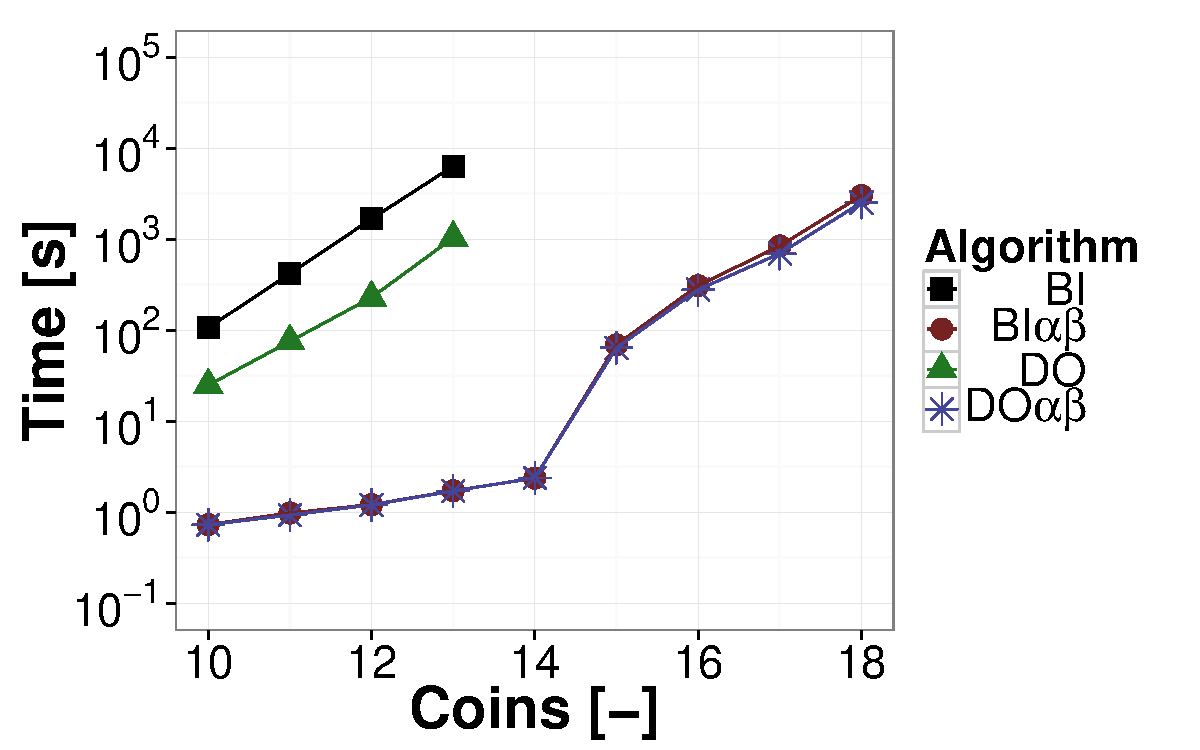
\includegraphics[width=1\textwidth]{figures/OZ-K4.pdf}\caption{}\label{fig:off:res:oz4}
	\end{subfigure}
	\begin{subfigure}{0.49\textwidth}
		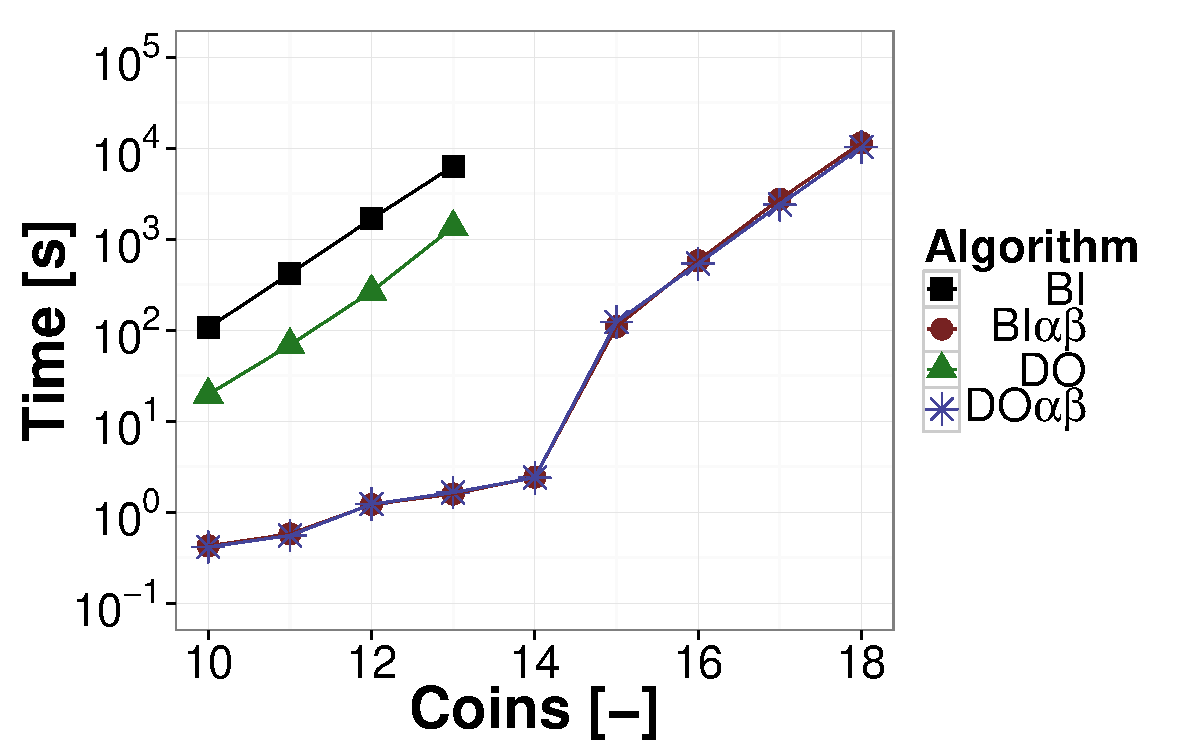
\includegraphics[width=1\textwidth]{figures/OZ-K4-BF.pdf}\caption{}\label{fig:off:res:oz4-bf}
	\end{subfigure}
\caption{Running times of exact algorithms on Oshi-Zumo with $K$ set to $4$ and increasing number of coins: subfigure (a) depicts the results for binary utilities, (b) depicts the results with point utilities.} \label{fig:off:res:oz}
\end{figure}

Many instances of the Oshi-Zumo game have Nash equilibria in pure strategies regardless on the type of utility function.
Although this does not hold for all the instances, the size of the subgames with pure NE are rather large and cause dramatic computation speed-up for both algorithms using serialized alpha-beta search.
If the game does not have equilibria in pure strategies, the mixed strategies are still required only near the root node and large end-games are solved using alpha-beta search.
Note that this is different to pursuit-evasion games, where mixed strategies were necessary close to the end of the game tree.
\reviewchange{
Figure~\ref{fig:off:res:oz} depicts the results with the parameter $K$ set to $4$ and for two different settings of utility function\footnote{\reviewchange{We have also performed the same experiments with $K$ set to $3$, but the conclusions were the same as in case $K=4$.}}; either a win-tie-lose utilities (left subfigure) or point utilities (right subfigure).}
In both cases, the graphs show the breaking point when the game stops having an equilibrium in pure strategies ($15$ coins and more for each player).
The advantage of $\biab$ and $\doab$ algorithms that exploit serialized variants of alpha-beta algorithms is dramatic.
We can see that both \textsc{BI} and \textsc{DO} scale rather badly.
The algorithms were able to scale up to $13$ coins in reasonable time.
For setting with $K=4$ and $13$ coins, it takes almost $2$ hours for \textsc{BI} to solve the game (the algorithm evaluates $1.5\times10^7$ nodes) regardless of the utility values.
\textsc{DO} improves the performance slightly (the algorithm evaluates $2.8\times10^6$ nodes in $17$ minutes \reviewchange{for the win-tie-lose utilities; the performance is slightly worse for point utilities: $5\times10^6$ nodes in $23$ minutes).}
Both $\biab$ and $\doab$, however, solved a single alpha-beta search on each serialization finding a pure NE.
Therefore, their performance is identical and it takes around $1.5$ seconds to solve the game for both types of utilities.
Although with an increasing number of coins the algorithms $\biab$ and $\doab$ need to find mixed Nash equilibria, their performance is very similar for both types of utilities.
\reviewchange{
As expected, the case with point utilities is more challenging and the algorithms scale worse -- for $18$ coins both algorithms solve the game with win-tie-lose utilities in approximately $1$ hour ($\biab$ in $50$ minutes, $\doab$ in $64$), it takes the algorithms around $3$ hours to solve the case with point utilities ($\biab$ in $191$ minutes, $\doab$ in $172$ minutes).
}

\begin{figure}[t!]
\centering
	\begin{subfigure}{0.85\textwidth}
		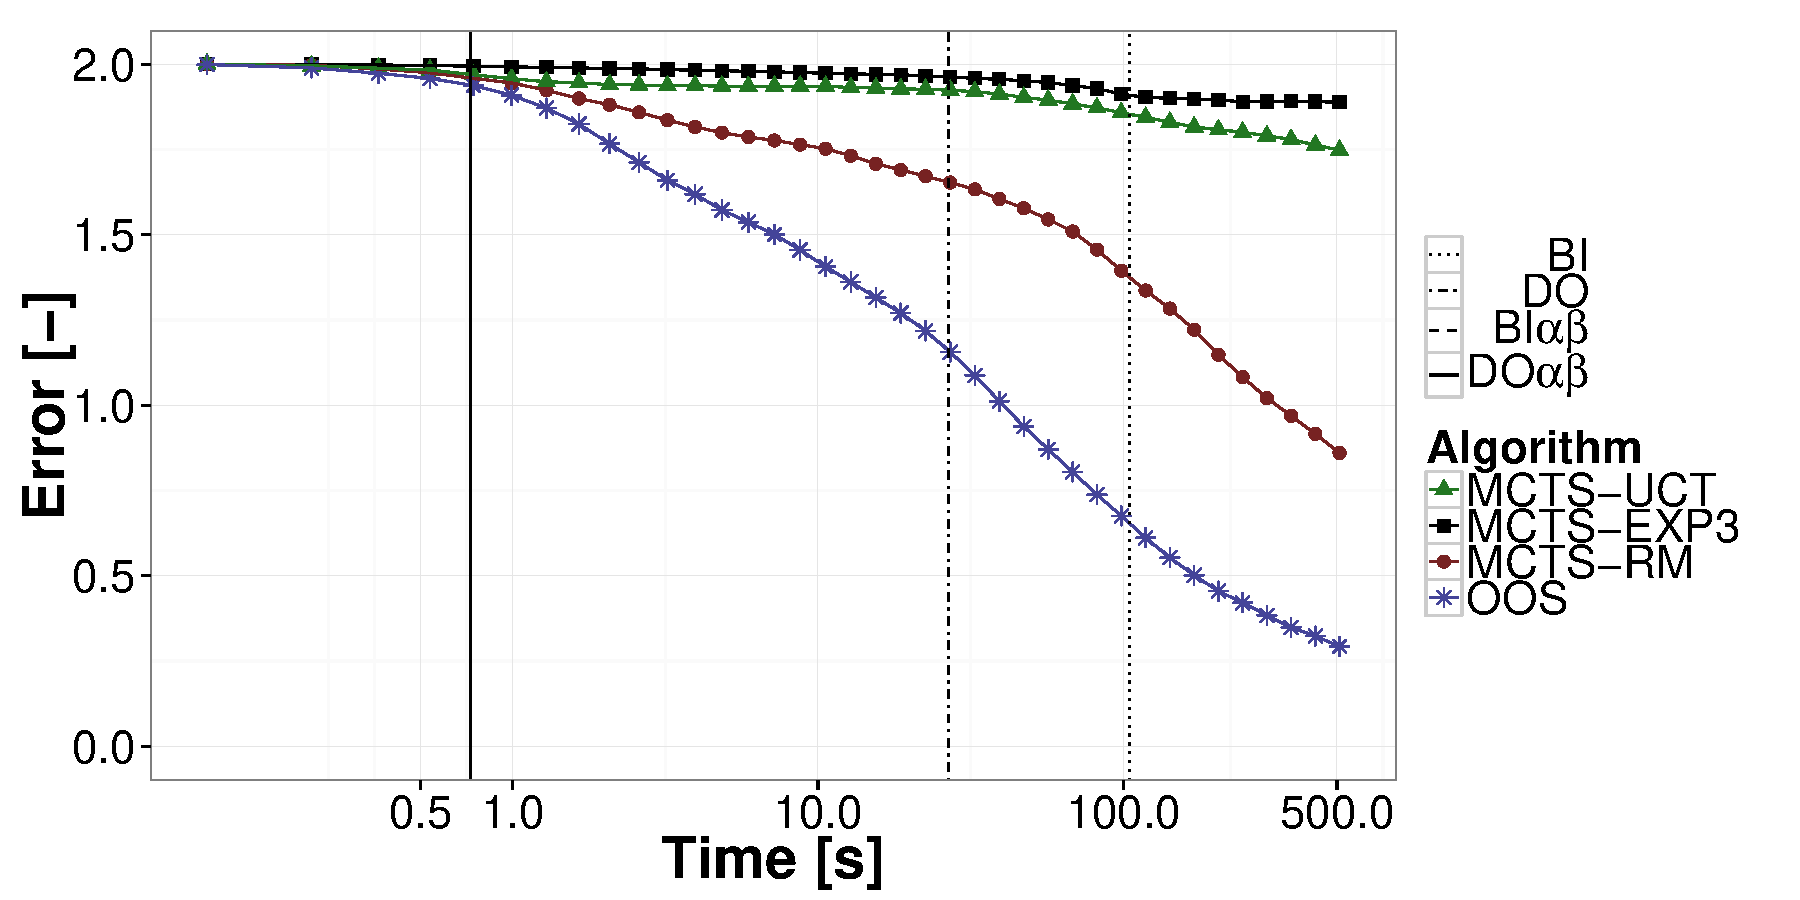
\includegraphics[width=1\textwidth]{figures/convergence-oz.pdf}
	\end{subfigure}
	\begin{subfigure}{0.85\textwidth}
		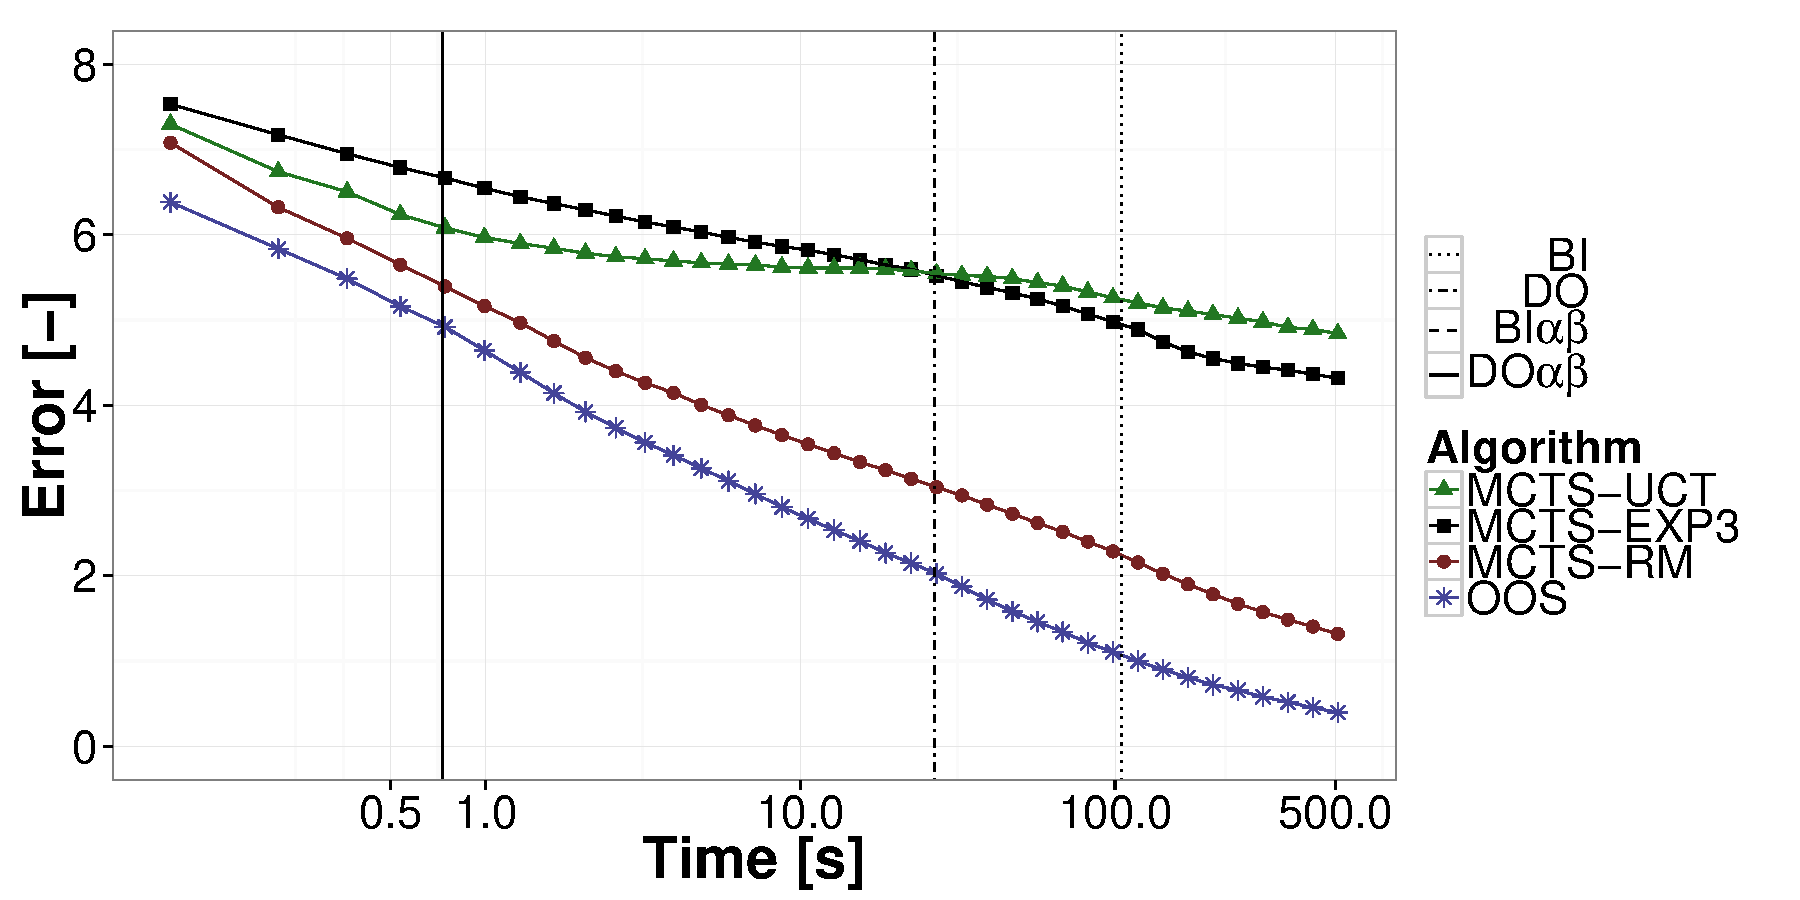
\includegraphics[width=1\textwidth]{figures/convergence-oz-bf.pdf}
	\end{subfigure}
\caption{Convergence of sampling algorithms on Oshi-Zumo game, with $10$ coins, $K=3$, and $M=1$. The vertical lines correspond to computation times of exact algorithms.
(Top) Oshi-Zumo with win-tie-lose utility values;
(Bottom) Oshi-Zumo with point utilities.} \label{fig:off:conv:oz}
\end{figure}

Turning to the sampling algorithms reveals that the game is difficult to approximate even in the win-tie-lose setting.
Figure~\ref{fig:off:conv:oz} depicts results for convergence of the sampling algorithms for the game with $10$ coins, $K$ set to $3$ and minimum bid set to $1$. This is an easy game for $\doab$ and $\biab$ with pure strategy and both of these algorithms are able to solve the game in less than a second ($0.73$). However, due to large branching factor for both players ($10$ actions at the root node for each player) all sampling algorithms converge extremely slowly. The performance of the algorithms in terms of iterations per second is similar to the previous games, however, OOS is slightly better in this case with $1.9\times10^5$ iterations per second compared to the second RM with $1.6\times10^5$ iterations per second.

As before, OOS is the best converging algorithm, however, in a given time limit ($500$ seconds) the reached error was only slightly below $0.3$ ($0.29$). On the other hand, all of the other sampling algorithms perform significantly worse -- RM ends with error slightly over $1$, UCT ($C=2$) with $1.50$, and Exp3 with $1.88$.
This confirms our findings from the previous experiment that increasing branching factor slows down the convergence rate.
Secondly, since there is a pure Nash equilibrium in this particular game configuration, the convergence of the algorithms is also slower since they essentially mix the strategy during the iterations in order to explore the unvisited parts of the game tree. Since none of the sampling algorithms can directly exploit this fact, their performance in offline solving games like Oshi-Zumo is not compelling. On the other hand, the existence of pure NE explains the better performance of UCT compared to Exp3 that is forced to explore more broadly.
\reviewchange{Moreover, convergence takes even more time in the point utility case, since the range of the utility values is larger.
OOS is again the fastest and converges to error $0.45$ within the time limit, RM to $1.41$, UCT ($C=4$) to $3.1$, and Exp3 $3.7$.}


\subsubsection{Random Games}
\begin{figure}[t!]
\centering
	\begin{subfigure}{0.49\textwidth}
		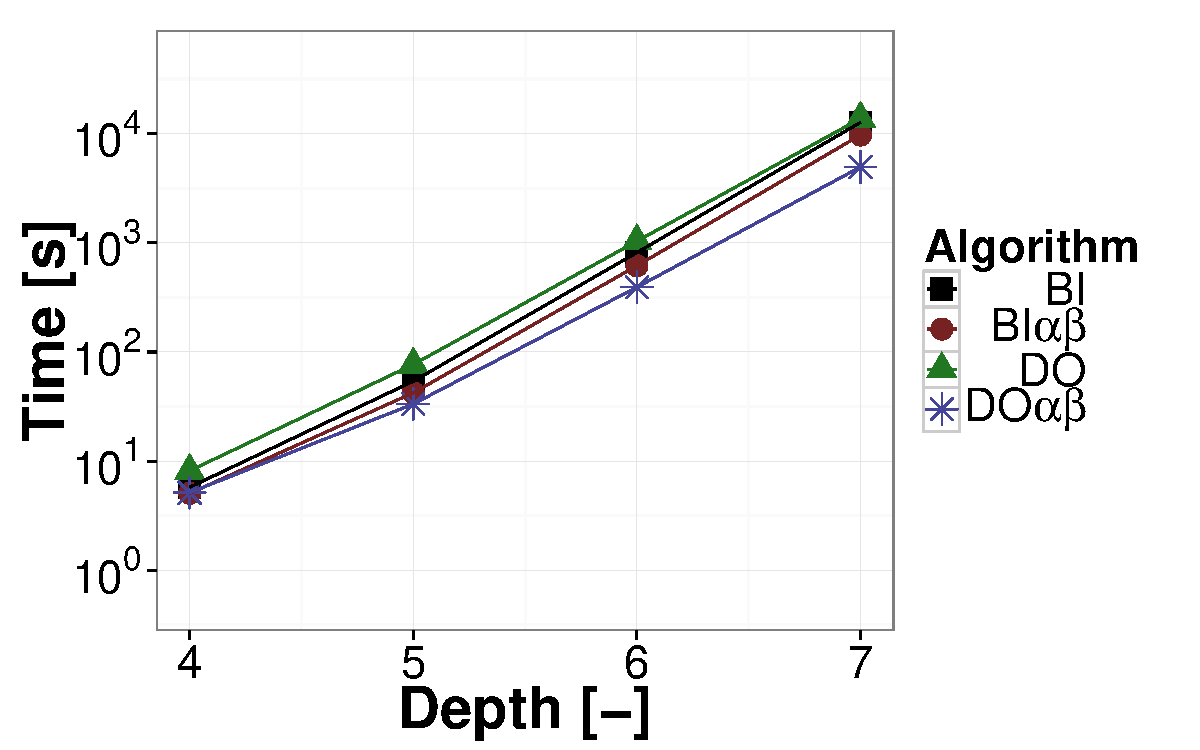
\includegraphics[width=1\textwidth]{figures/RG-BF4-BIN-FALSE.pdf}\caption{}\label{fig:off:res:rgbf4}
	\end{subfigure}
	\begin{subfigure}{0.49\textwidth}
		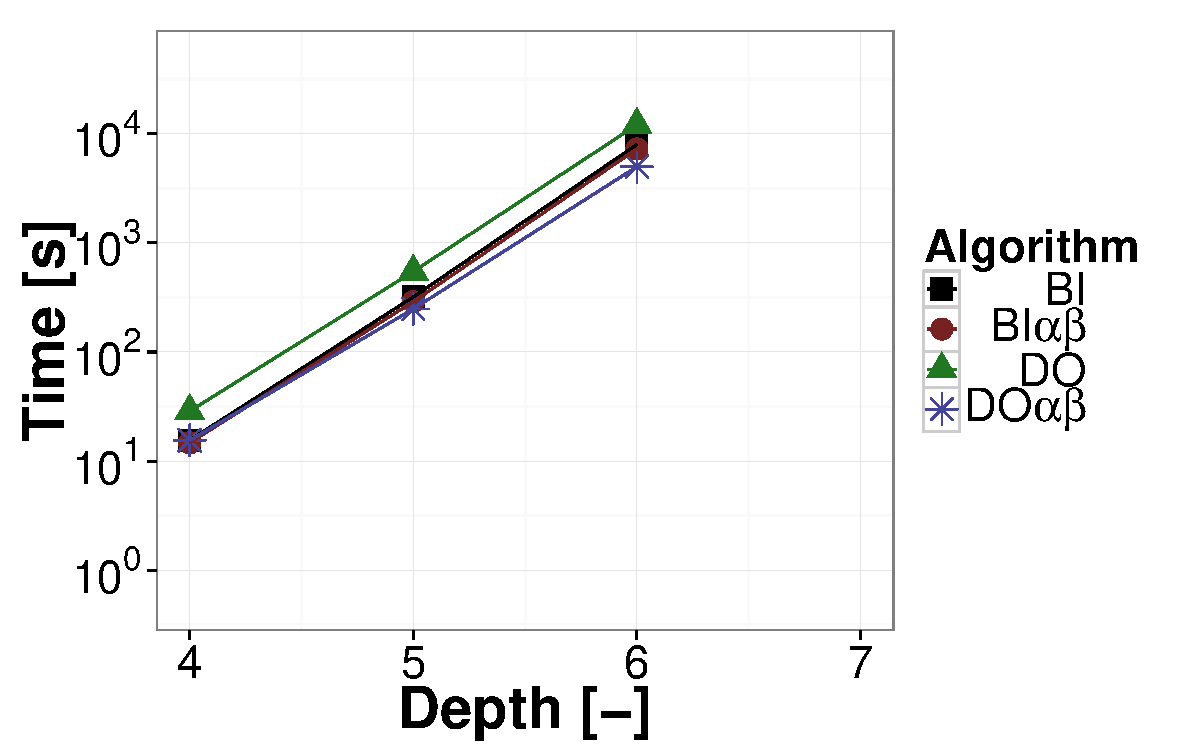
\includegraphics[width=1\textwidth]{figures/RG-BF5-BIN-FALSE.pdf}\caption{}\label{fig:off:res:rgbf5}
	\end{subfigure}
\caption{Running times of exact algorithms on randomly generated games with increasing depth: subfigure (a) depicts the results with branching factor set to $4$ actions for each player, (b) depicts the results with branching factor $5$.} \label{fig:off:res:rg}
\end{figure}

In the first variant of the randomly generated games we used games with utility values randomly drawn from a uniform distribution $[0,1]$.
Such games represent an extreme case, where neither alpha-beta search, nor double-oracle algorithm can save much computation time, since each action can lead to arbitrarily good or bad terminal state.
In these games, \textsc{BI} algorithm is typically the fastest.
Even though both $\biab$ and $\doab$ evaluate marginally fewer nodes ($\approx90\%$), the overhead of the algorithms (repeated calculation of alpha-beta algorithm, repeatedly solving linear programs, etc.) causes slower runtime performance in this case.

However, completely random games are rarely instances that need to be solved in practice.
The situation changes, when we use the intuition of good and bad moves and thus add correlation to the utility values.
Figure~\ref{fig:off:res:rg} depicts the results for two different branching factors $4$ and $5$ for each player and increasing depth.
The results show that $\doab$ outperforms all remaining algorithms, although the difference is rather small (still statistically significant).
On the other hand, \textsc{DO} without serialized alpha-beta is not able to outperform \textsc{BI}.
This is most likely caused by a larger support in mixed subgame equilibria that cause enumerating most of the actions by the double-oracle algorithm.
Moreover, this is also demonstrated by the performance of $\biab$ that is only slightly better compared to \textsc{BI}.

The fact that serialized alpha-beta is less successful in randomly generated games is noticeable also when comparing the number of evaluated nodes.
For case with branching factor set to $4$ for both players, and depth $7$, \textsc{BI} evaluates almost $1.8\times10^7$ nodes in almost $3.5$ hours, while $\biab$ evaluates more than $\approx1\times10^7$ nodes in almost $3$ hours.
\textsc{DO} evaluates even more nodes compared to $\biab$ ($\approx1.2\times10^7$) and it is slower compared to both \textsc{BI} and $\biab$.
Finally, $\doab$ evaluates $\approx2\times10^6$ nodes on average and it takes the algorithm slightly over $80$ minutes.

\begin{figure}[t!]
\centering
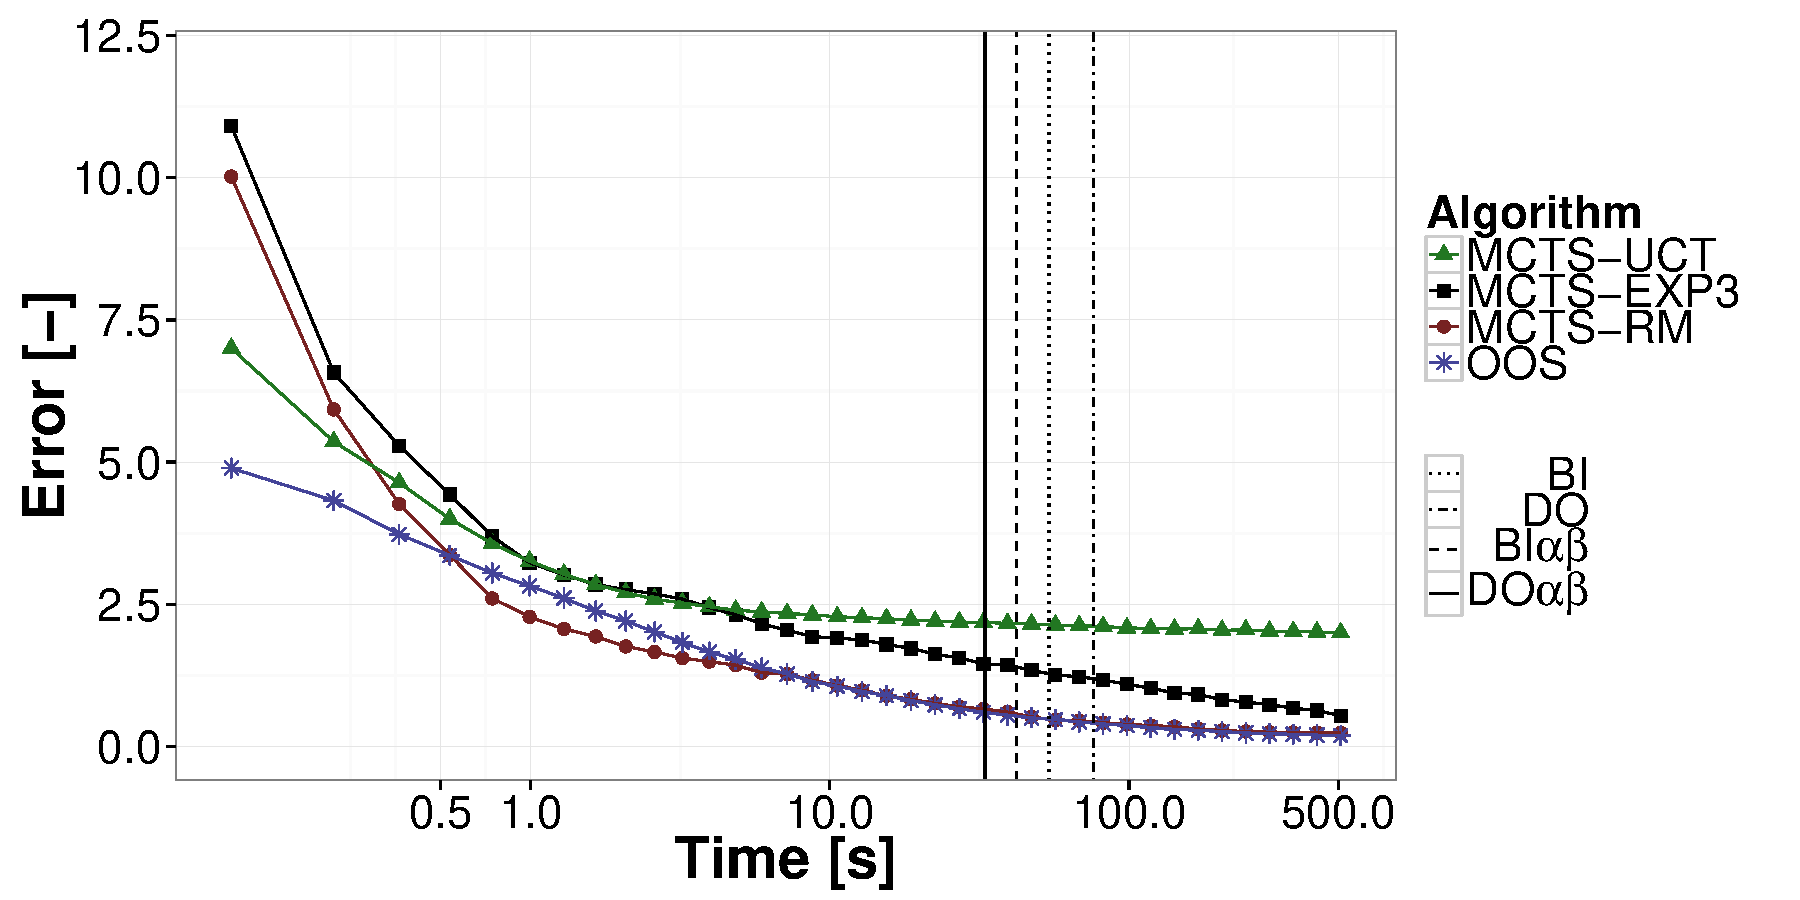
\includegraphics[width=0.85\textwidth]{figures/convergence-rg.pdf}
\caption{Convergence of sampling algorithms on random game with branching factor $4$ and depth $5$. The vertical lines correspond to computation times of exact algorithms.} \label{fig:off:conv:rg}
\end{figure}

Figure~\ref{fig:off:conv:rg} depicts the results for convergence of the sampling algorithms for the random game with correlated utility values, branching factor set to $4$ and depth $5$.
The number of iterations per second is similar to Goofspiel, with Exp3 being the exception able to achieve more than $6.5\times10^4$ iterations per second, which is still significantly the lowest number of iterations.
Interestingly, there is a much less difference between the performance of the sampling algorithms in this game.
Since these games are generally more mixed (\ie NE require to use mixed strategies in many states of the game), they are much more suitable for the sampling algorithms.
OOS can be considered a winner in this setting, however, the performance of RM is very similar.
Again, since the game is more mixed, Exp3 outperforms UCT in the longer run.
Exploration constant for UCT was set to 12 due to larger utility variance in this setting.

\subsubsection{Tron}

\begin{figure}[t!]
\centering
	\begin{subfigure}{0.49\textwidth}
		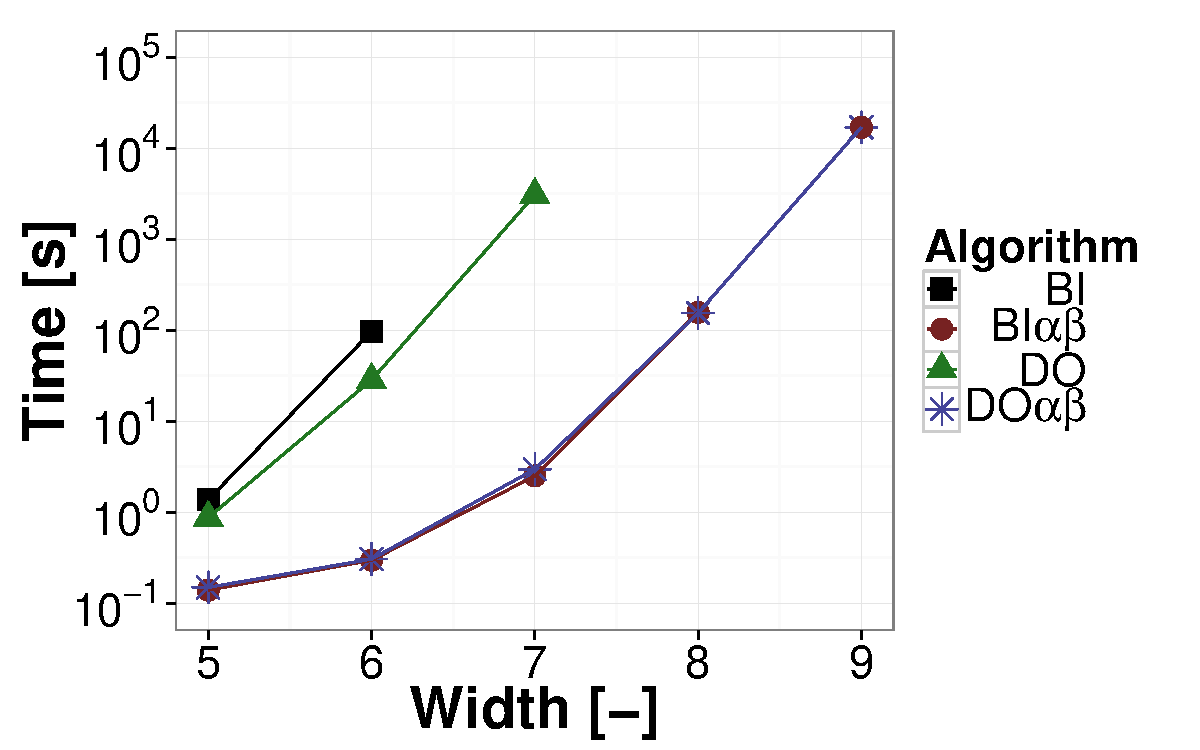
\includegraphics[width=1\textwidth]{figures/Tron-1.pdf}\caption{}\label{fig:off:res:tron1}
	\end{subfigure}
	\begin{subfigure}{0.49\textwidth}
		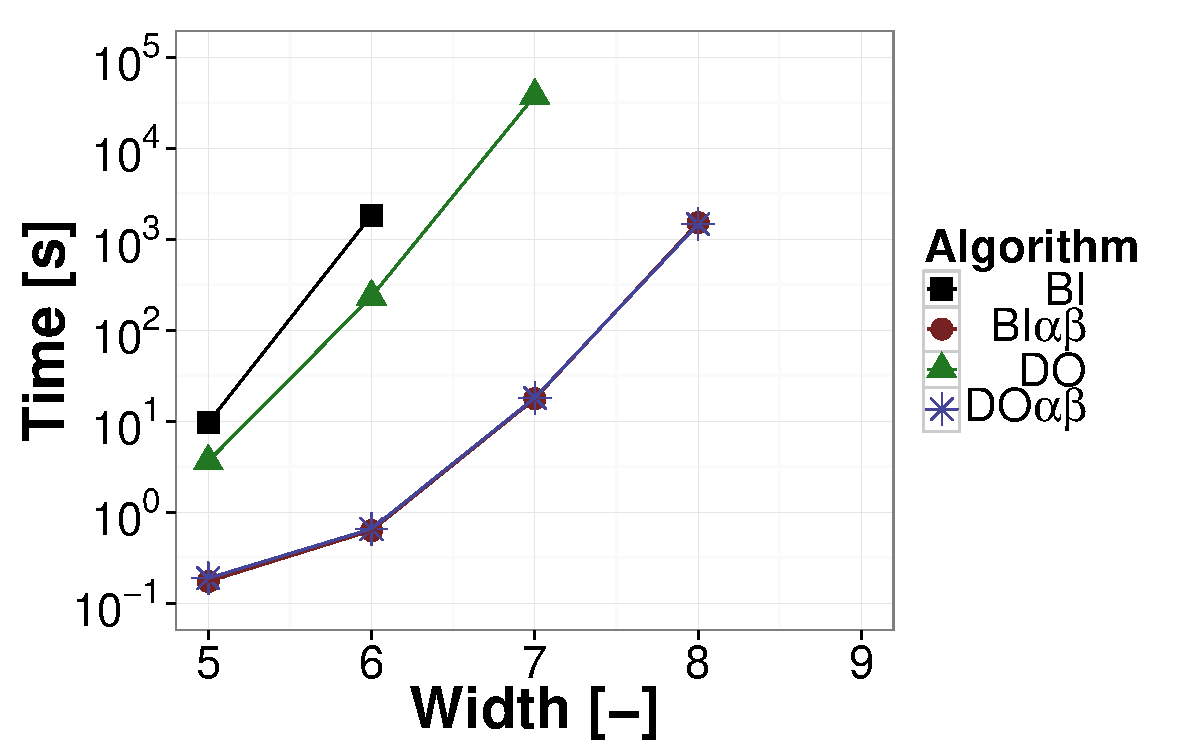
\includegraphics[width=1\textwidth]{figures/Tron-2.pdf}\caption{}\label{fig:off:res:tron2}
	\end{subfigure}
\caption{Running times of exact algorithms on Tron with increasing $width$ of the graph: subfigure (a) depicts the results with $height$ of the graph set to $width - 1$, (b) depicts the results with $height = width$.} \label{fig:off:res:tron}
\end{figure}

Performance of exact algorithms in Tron is affected by the fact that pure NE exist in all smaller instances \reviewchange{
(the results are depicted for two different ratios of dimensions of the grid in Figure~\ref{fig:off:res:tron})}.
Therefore, $\biab$ and $\doab$ are essentially the same since serialized alpha-beta is able to solve the game.
Moreover, since the size of the game increases dramatically with increasing size of the grid (the longest branch of the game tree has $\left(0.5\cdot w\cdot l - 1\right)$ joint actions, where $w$ and $l$ are dimensions of the grid), the performance of standard BI is very poor.
While BI is able to solve the grid $5\times6$ in $96$ seconds, it takes around $30$ minutes to solve $6\times6$ grid.
By comparison, DO solves the $6\times6$ instance in $235$ seconds, and both $\biab$ and $\doab$ in $0.6$ seconds.
\reviewchange{
$\biab$ and $\doab$ scale much better and the largest graph these algorithms solved had size $9\times9$ taking almost $2$ days to solve.
}

\begin{figure}[t]
\centering
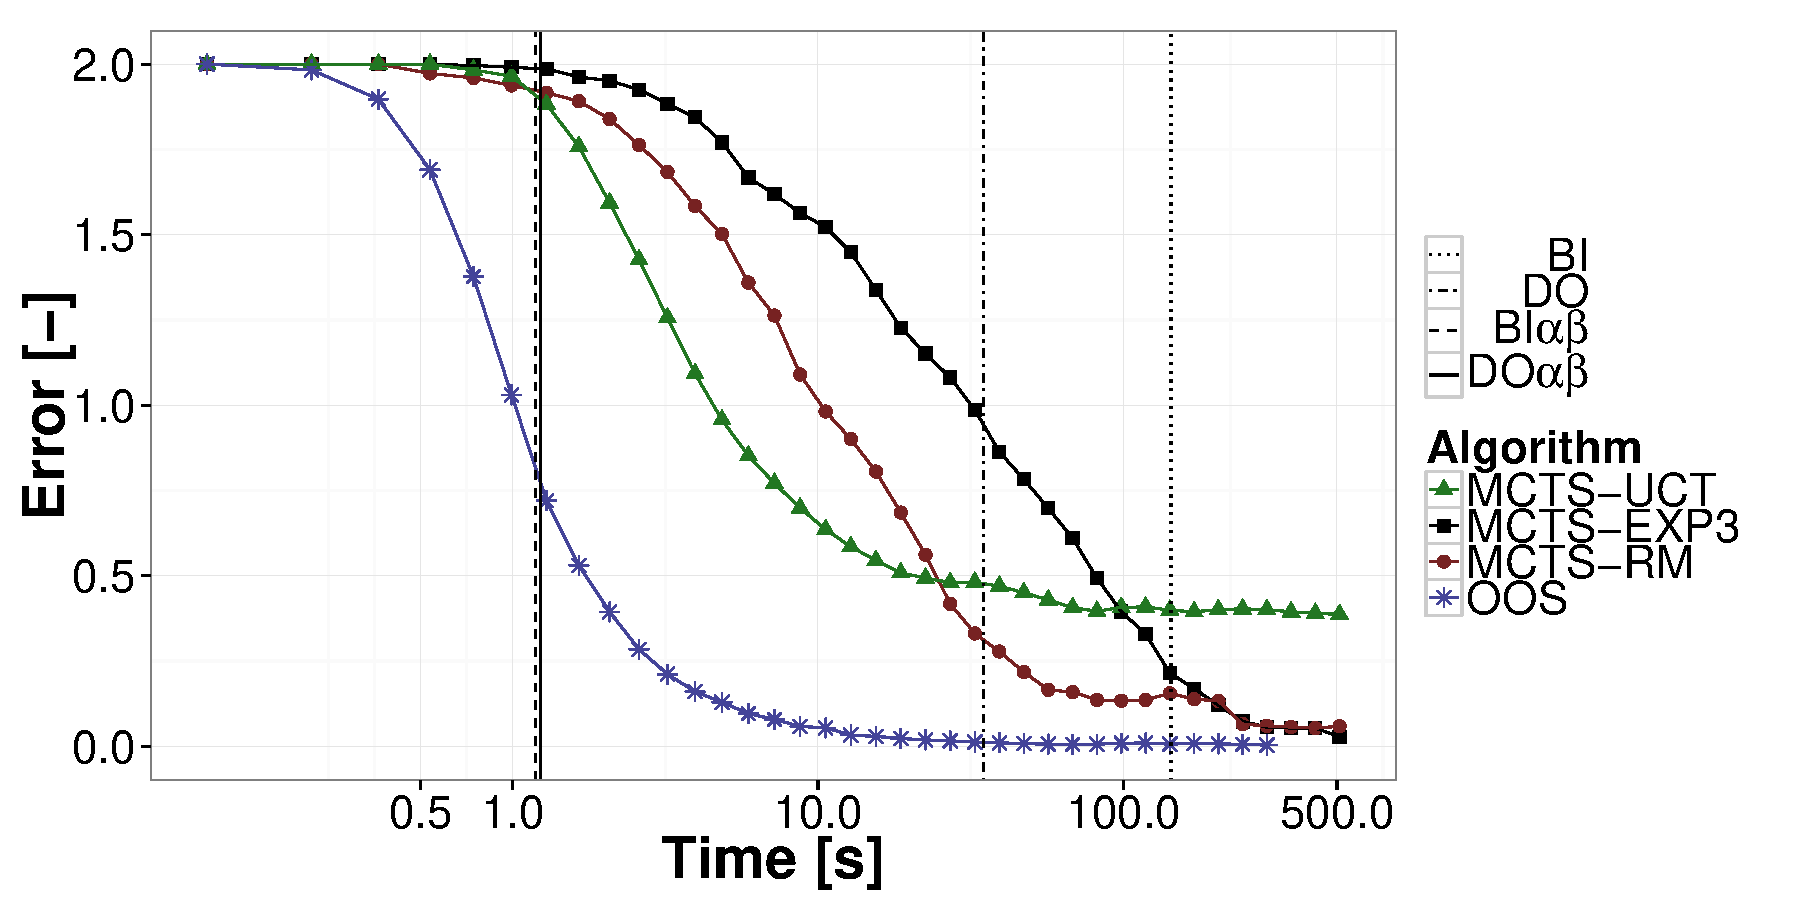
\includegraphics[width=0.85\textwidth]{figures/convergence-tron.pdf}
\caption{Convergence comparison of different sampling algorithms on Tron on grid $5\times6$. The vertical lines correspond to computation times for exact algorithms.} \label{fig:off:conv:tron}
\end{figure}

The size of the game tree in Tron also causes slow convergence for sampling algorithms.
This is apparent also in the number of iterations that is slightly slower for the algorithms.
OOS is the fastest performing $1.3\times 10^5$ iterations per second, RM achieves $1.2\times 10^5$ iterations, UCT only $8\times10^4$, and Exp3 is again the slowest with $7.8\times10^4$ iterations per second.
Figure~\ref{fig:off:conv:tron} depicts the results for the grid $5\times6$.
Consistently with the previous results, OOS performs the best and it is able to converge to very close to exact solution in $300$ seconds.
Similarly, both RM and Exp3 are again eventually able to converge to a very small error, however, it take them more time and in the time limit they achieve error $0.05$, or $0.02$ respectively.
Finally, UCT ($C=5$) performs reasonably well during the first $10$ seconds, where the exploitability is better than both RM and Exp3.
This is most likely due to existence pure NE, however, the length of the game tree prohibits UCT to converge and the best error the algorithm was able to achieve in the time limit was equal to $0.68$.

\subsubsection{Summary of Offline Equilibrium Computation Experiments}

The offline comparison of the algorithms offers several conclusions.
Among the exact algorithms, $\doab$ is clearly the best algorithm, since it typically outperforms all other algorithms (especially in pursuit-evasion games and random games). Although for smaller games (\eg Goofspiel with $5$ cards)  $\biab$ can be slightly faster, this difference is not significant and $\doab$ is never significantly slower compared to $\biab$.

Among the sampling algorithms, OOS is the clear winner since it is often able to quickly converge to a very small error and significantly outperforms all variants of MCTS.
On the other hand, comparing OOS and $\doab$, the exact $\doab$ algorithm is always faster and it is able to find an exact solution much faster compared to OOS.
Moreover, $\doab$ has significantly lower memory requirements since it is a depth-first search algorithm and does not use any form of global cache, while OOS iteratively constructs the game tree in memory.

\subsection{Online Search}

We now compare the performance of the algorithms in head-to-head matches in the same games as we used in the offline equilibrium computation experiments, but we use a much larger instances of these games. \reviewchange{Each algorithm has a strictly limited computation time per move set to 1 second.} After this time, the algorithm outputs an action to be played in the current game state, receives information about the action selected by its opponent, and the game proceeds to the next state. As described in Section~\ref{sec:online}, all algorithms keep results of previous computations and do not start form scratch in the next state. \reviewchange{We have also performed a large set of experiments with 5 seconds of computation time per move, however, the results are very similar to the results with 1 second per move. Therefore, we presents the results with 1 second in details and only comment on the 5 seconds results where additional time leads to an interesting difference.}

We compare all of the approximative sampling algorithms and $\doab$ as a representative of backward induction algorithms, because it was clearly the fastest algorithm in all of the considered games.
Finally, we also included random player (denoted RAND) into the tournament to confirm that the algorithms choose better strategies than the simple random game play.
%In the following experiments, we aim to identify the algorithms that are most suitable in the online search setting and study the relation of the performance in approximating the equilibrium in the offline setting and actual game playing performance in the matches.
We report expected rewards and win rates of the algorithms, in which a tie is counted as half win.
\reviewchange{The parameters of the algorithms are tuned for each domain separately.
We first present the comparison of different algorithms and we discuss the influence of the parameters in Subsection~\ref{sec:eval:online:tuning}.}

\reviewchange{In this subsection, we show cross tables of each algorithm (on the row) matched up against each competitor algorithm (on the column).}
Each entry represents a mean of at least $1000$ matches with the half of the width of the $95\%$ confidence interval in brackets, \eg $52.9(0.3)$ refers to $52.9\% \pm 0.3\%$.
\reviewchange{The result shown is the win rate for the row player, so as an example in the standard game of Goofspiel (top of Table~\ref{fig:matches:goof}) $\doab$ wins $67.2 \% \pm 1.4 \%$ of games against the random player.
All evaluated games, besides the pursuit evasion game, are symmetric from the position of the first and the second player. We made even the random games symmetric by always playing matches on the same game instance in pairs with alternating players' positions. However, for easier comparison of the algorithms, we mirror the same results to both fields corresponding to a pair of players in the cross tables.
}

\subsubsection{Goofspiel}

\begin{table}
\centering
\begin{scriptsize}

Goofspiel: 13 cards, stochastic sequence of cards, win rate
\begin{tabular}{|r|cccccc|}\hline
&$\doab$&OOS(0.2)&UCT(0.6)&EXP3(0.3)&RM(0.1)&RAND\\\hline
$\doab$&$\bullet$&26.6(2.7)&36.0(2.9)&26.1(2.7)&25.9(2.7)&67.2(1.4)\\
OOS&73.4(2.7)&$\bullet$&\textbf{51.2(2.1)}&52.5(2.2)&47.5(3.0)&81.4(1.7)\\
UCT&64.0(2.9)&48.8(2.1)&$\bullet$&55.6(2.1)&\textbf{49.7(3.0)}&77.3(1.8)\\
EXP3&73.8(2.7)&47.5(2.2)&44.4(2.1)&$\bullet$&41.1(3.0)&\textbf{86.1(1.5)}\\
RM&\textbf{74.1(2.7)}&\textbf{52.5(3.0)}&50.3(3.0)&\textbf{58.9(3.0)}&$\bullet$&85.2(2.2)\\
RAND&32.8(1.4)&18.6(1.7)&22.7(1.8)&13.9(1.5)&14.8(2.2)&$\bullet$\\
\hline
\end{tabular}

Goofspiel: 13 cards, known sequence of cards, win rate
\begin{tabular}{|r|cccccc|}\hline
&$\doab$&OOS(0.3)&UCT(0.8)&EXP3(0.2)&RM(0.1)&RAND\\\hline
$\doab$&$\bullet$&28.2(2.8)&35.0(2.9)&30.1(2.8)&31.5(2.8)&67.2(2.9)\\
OOS&\textbf{71.8(2.8)}&$\bullet$&46.2(3.0)&51.8(3.0)&\textbf{49.6(3.0)}&83.8(2.3)\\
UCT&65.0(2.9)&\textbf{53.8(3.0)}&$\bullet$&\textbf{57.1(2.9)}&48.6(2.9)&79.5(2.5)\\
EXP3&70.0(2.8)&48.2(3.0)&42.9(2.9)&$\bullet$&46.5(3.0)&\textbf{85.8(2.1)}\\
RM&68.5(2.8)&50.4(3.0)&\textbf{51.4(2.9)}&53.5(3.0)&$\bullet$&84.2(2.2)\\
RAND&32.8(2.9)&16.2(2.3)&20.5(2.5)&14.2(2.1)&15.8(2.2)&$\bullet$\\
\hline
\end{tabular}

Goofspiel: 13 cards, known sequence of cards, point utilities
\begin{tabular}{|r|cccccc|}\hline
&$\doab$&OOS(0.3)&UCT(0.8)&EXP3(0.2)&RM(0.1)&RAND\\\hline
$\doab$&$\bullet$&-7.74(0.94)&-8.89(0.91)&-6.45(0.94)&-7.88(0.96)&6.67(0.99)\\
OOS&7.74(0.94)&$\bullet$&1.19(0.78)&3.27(0.82)&\textbf{0.35(0.76)}&14.42(0.96)\\
UCT&\textbf{8.89(0.91)}&-1.19(0.78)&$\bullet$&1.72(0.80)&-1.94(0.73)&13.30(1.00)\\
EXP3&6.45(0.94)&-3.27(0.82)&-1.72(0.80)&$\bullet$&-5.02(0.79)&\textbf{14.79(0.97)}\\
RM&7.88(0.96)&\textbf{-0.35(0.76)}&\textbf{1.94(0.73)}&\textbf{5.02(0.79)}&$\bullet$&14.20(0.98)\\
RAND&-6.67(0.99)&-14.42(0.96)&-13.30(1.00)&-14.79(0.97)&-14.20(0.98)&$\bullet$\\
\hline
\end{tabular}
\end{scriptsize}
\caption{Results of head-to-head matches in Goofspiel variants with exploration parameter settings indicated in the table headers.}\label{fig:matches:goof}
\end{table}

\reviewchange{In head-to-head comparison, our focus is primarily on the standard Goofspiel with 13 cards and chance nodes. Additionally, for the sake of consistency with the offline results, we also evaluate the variant with a fixed known sequence of cards. The full game has more than $2.4\times 10^{29}$ leaf nodes and the variant with fixed sequence has still more than $3.8\times 10^{19}$ leaf nodes. The results are presented in Table~\ref{fig:matches:goof}, where the top table shows the win rates of the algorithms in the full game and the other two tables the win rates and expected number of points gained by the algorithms in the game with a fixed point card sequence. The results for the know card sequence are the mean of $10$ fixed random sequences. For each table, the algorithms were set up to optimize the presented measure (\ie win rate or points) and the exploration parameters were tuned to the values presented in the header of the table.

First, we can see that finding a good strategy in Goofspiel is difficult for all the algorithms.
This is noticeable thanks to the results of RAND player, that performs reasonably well
(RAND typically loses almost every match in all the remaining game domains).
Next, we analyze the results of the $\doab$ algorithms compared to the sampling algorithms.
The results show that even though $\doab$ uses a domain-specific heuristic evaluation function, it does not win significantly against any of the sampling algorithms that does not use any domain knowledge.
The difference is always statistically significant with a large margin.
When optimizing win percentage, $\doab$ loses the least against UCT while in optimizing the expected reward, UCT performs significantly the best.
The performance of the other sampling algorithms is very similar against $\doab$, with Exp3 winning the least in reward optimization.

We compare the sampling algorithms in the game variants in the order of the presented tables.
The differences in the performance of the sampling algorithms are relatively small among each other.
They are more noticeable mainly against the weaker players, which are outperformed by all sampling algorithms.
In the game with stochastic point card sequence, OOS, UCT and RM make approximately $10 \times 10^3$ iterations in the 1 second time limit in the root of the game. Exp3 is slightly slower with $8 \times 10^3$ iterations.
The best algorithm in this game variant is RM, which wins against all other sampling algorithms and wins most often against $\doab$ and Exp3.
The second best algorithm is OOS, which loses only against RM and Exp3 is the weakest algorithm losing against all other sampling algorithms.

The sampling algorithms in the second game variant (without chance) perform 
the same number of samples as in the first variant, with the exception of UCT, which performs $12 \times 10^3$ iterations per second.
However, they build a considerably deeper search trees, since the game tree is less wide.
The exploration parameters were tuned to slightly larger numbers, which indicate that more exploration is beneficial in smaller games.
The results are similar to the previous game variant.
RM is still winning against all opponents, but it is not able to win more often against weaker players, which is consistent with playing close to a Nash equilibrium.
UCT loses only against RM in this variant and it significantly outperforms OOS and Exp3.
This indicates that UCT was able to better focus on the relevant part of the smaller game, which is supported also by larger number of simulations, which can be caused by smaller random simulations after leaving the part of the search tree stored in memory.

When players optimize the expected reward, the differences between the algorithms are larger. 
We can see that RM and OOS perform significantly better than UCT and Exp3.
OOS wins against all opponents and RM loses only against OOS.
An important reason behind the decrease of the performance of Exp3 is that after normalizing the reward to unit interval, the important differences in values for reasonably good strategies become much smaller, which slows down the learning of the algorithm.
UCT compensates the range of the rewards by the choice of the exploration parameter, but different nodes would benefit from different exploration parameters, which causes more inefficiencies with more variable rewards.
An important advantage of OOS and RM is that their behavior is practically independent form the range of payoffs.

In summary, RM is the only algorithm that did not lose significantly against any other sampling algorithm in any other game variant and often wins significantly.
Exp3 is overall the weakest algorithm, losing to all other algorithm in all Goofspiel variants.
Interestingly, Exp3 always performs the best against the random player, which indicates slower convergence to more sophisticated strategies.}

\subsubsection{Oshi-Zumo}

\begin{table}[t!]
\centering
\begin{scriptsize}

Oshi Zumo: 50 coins, $K=3$, win rate
\begin{tabular}{|r|cccccc|}\hline
&$\doab$&OOS(0.2)&UCT(0.4)&EXP3(0.8)&RM(0.1)&RAND\\\hline
$\doab$&$\bullet$&\textbf{79.2(2.5)}&\textbf{77.6(2.6)}&\textbf{84.8(2.2)}&\textbf{84.0(2.3)}&98.8(0.5)\\
OOS&20.9(2.5)&$\bullet$&27.7(2.6)&57.1(2.1)&51.2(2.1)&98.9(0.4)\\
UCT&\textbf{22.4(2.6)}&72.3(2.6)&$\bullet$&83.0(2.0)&70.3(2.6)&\textbf{99.9(0.2)}\\
EXP3&15.2(2.2)&42.9(2.1)&17.0(2.0)&$\bullet$&44.5(2.8)&98.5(0.5)\\
RM&16.0(2.3)&48.8(2.1)&29.6(2.6)&55.5(2.8)&$\bullet$&99.0(0.4)\\
RAND&1.2(0.5)&1.1(0.4)&0.1(0.2)&1.5(0.5)&1.0(0.4)&$\bullet$\\
\hline
\end{tabular}

Oshi Zumo: 50 coins, $K=3$, point utilities
\begin{tabular}{|r|cccccc|}\hline
&$\doab$&OOS(0.2)&UCT(0.4)&EXP3(0.8)&RM(0.1)&RAND\\\hline
$\doab$&$\bullet$&\textbf{2.33(0.19)}&\textbf{2.27(0.20)}&3.62(0.10)&\textbf{2.85(0.17)}&3.65(0.09)\\
OOS&-2.33(0.19)&$\bullet$&-0.53(0.19)&3.46(0.10)&0.25(0.20)&3.87(0.05)\\
UCT&\textbf{-2.27(0.20)}&0.53(0.19)&$\bullet$&\textbf{3.68(0.07)}&0.58(0.17)&\textbf{3.93(0.02)}\\
EXP3&-3.62(0.10)&-3.46(0.10)&-3.68(0.07)&$\bullet$&-3.53(0.09)&1.31(0.17)\\
RM&-2.85(0.17)&-0.25(0.20)&-0.58(0.17)&3.53(0.09)&$\bullet$&3.87(0.04)\\
RAND&-3.65(0.09)&-3.87(0.05)&-3.93(0.02)&-1.31(0.17)&-3.87(0.04)&$\bullet$\\
\hline
\end{tabular}

Oshi Zumo: 50 coins, $K=3$, win rate, evaluation function
\begin{tabular}{|r|cccccc|}\hline
&$\doab$&OOS(0.3)&UCT(0.8)&EXP3(0.8)&RM(0.1)&RAND\\\hline
$\doab$&$\bullet$&63.0(2.1)&11.8(1.3)&52.9(2.2)&61.7(2.1)&98.6(0.5)\\
OOS&37.0(2.1)&$\bullet$&24.8(1.9)&33.4(2.0)&43.6(2.1)&99.6(0.3)\\
UCT&\textbf{88.2(1.3)}&\textbf{75.2(1.9)}&$\bullet$&\textbf{80.5(1.7)}&\textbf{71.1(2.0)}&\textbf{99.8(0.2)}\\
EXP3&47.1(2.2)&66.6(2.0)&19.5(1.7)&$\bullet$&58.7(2.1)&98.7(0.5)\\
RM&38.3(2.1)&56.4(2.1)&\textbf{28.9(2.0)}&41.3(2.1)&$\bullet$&99.6(0.3)\\
RAND&1.4(0.5)&0.4(0.3)&0.2(0.2)&1.3(0.5)&0.4(0.3)&$\bullet$\\
\hline
\end{tabular}
\end{scriptsize}
\caption{Results of head-to-head matches in Oshi-Zumo variants with exploration parameter settings indicated in the header. In the first two tables only $\doab$ uses a heuristic evaluation function and in the third table all algorithms use the evaluation function.}\label{fig:matches:oz}
\end{table}

In Oshi-Zumo, we use the setting with 50 coins, $2\cdot 3 + 1 = 7$ fields of the board (i.e., $K=3$), and minimal bet of 1.
The size of the game is large with strictly more than $10^{15}$ leaves (number of choices of a single player in the game; hence, square of this number is the upper bound on the number of leaves) and 50 actions for each player in the root.

\reviewchange{The results are depicted in Table~\ref{fig:matches:oz}. As in the case with Goofspiel, we show the results for both win rate as well as with points utilities. Moreover, our evaluation function in Oshi-Zumo is much more accurate than the one in Goofspiel and $\doab$ is clearly outperforming all sampling algorithms when they do not use any domain specific knowledge. Therefore we also run the experiments, where the sampling algorithms also used evaluation function instead of random rollout simulation.}

%In this game, the evaluation function used by $\doab$ is much stronger than in Goofspiel and all the sampling algorithms without domain specific knowledge perform poorly against this algorithm (see first two tables in Table~\ref{fig:matches:oz}). The loss is even higher with 5 seconds per move. UCT and OOS perform better against $\doab$ than RM and Exp3.

In the offline experiment (Figure~\ref{fig:off:conv:oz}), none of the sampling algorithms was able to converge anywhere close to the equilibrium in short time. Moreover, the game used in the offline experiments was orders of magnitude smaller (there were only $10$ coins for each player).
In spite of the negative results in the offline experiments, all sampling algorithms are able to find reasonably good strategy.
UCT is clearly the strongest sampling algorithm in all variants.
In the win rate setting, the strongest opponent of UCT among the sampling algorithms is RM (UCT wins 70.3\% of games), following by OOS performing only slightly worse (UCT wins 72.3\% of games).
Finally, Exp3 is clearly the weakest of all sampling algorithms.
A possible reason may be that Exp3 manages to perform around $2.5 \times 10^3$ iterations per second in the root, while the other algorithms perform ten times more. 
This is caused by the quadratic dependence of its computational complexity on the number of actions, which is relatively high in this game.
\reviewchange{The situation remains similar when the algorithms optimize the point utilities.}

% Because of high quality of the evaluation function in this game, we performed experiments where the rollout simulation was replaced with the evaluation function. 
We now turn to experiments with the evaluation function, results of which are presented in the third table of Table~\ref{fig:matches:oz}.
The results show that the quality of play of all sampling algorithms is significantly improved.
With this modification, UCT already significantly outperforms all algorithms including $\doab$.
$\doab$ is the second best and still winning over the remaining sampling algorithms.
Exp3 benefits from the evaluation function more than OOS and RM, which are relatively weaker with the evaluation function.

The reason UCT performs well in this game is that the game mostly requires pure strategies, rather then precise mixing between multiple strategies (see Subsection~\ref{sec:eval:domains}). UCT is able to quickly disregard other actions, if a single action is optimal.
\vlisy{evaluation function generally helps significantly to all algorithms, but can make significant changes in ranking of the algorithms} 

\subsubsection{Random Games}

\begin{table}
\centering
\begin{scriptsize}

\begin{tabular}{|r|cccccc|}\hline
&$\doab$&OOS(0.1)&UCT(1.5)&EXP3(0.6)&RM(0.3)&RAND\\\hline
$\doab$&$\bullet$&57.4(2.9)&\textbf{49.6(2.8)}&53.4(2.8)&51.3(2.8)&88.8(1.8)\\
OOS&42.6(2.9)&$\bullet$&33.5(2.5)&43.5(2.7)&42.5(2.8)&85.0(2.4)\\
UCT&\textbf{50.4(2.8)}&\textbf{66.5(2.5)}&$\bullet$&\textbf{67.4(2.5)}&\textbf{55.7(2.6)}&95.9(1.2)\\
EXP3&46.6(2.8)&56.5(2.7)&32.6(2.5)&$\bullet$&42.9(2.7)&\textbf{96.0(1.1)}\\
RM&48.7(2.8)&57.5(2.8)&44.3(2.6)&57.1(2.7)&$\bullet$&93.1(1.5)\\
RAND&11.2(1.8)&15.0(2.4)&4.1(1.2)&4.0(1.1)&6.9(1.5)&$\bullet$\\
\hline
\end{tabular}

\end{scriptsize}
\caption{Win-rate in head-to-head matches of Random games with 5 actions for each player in each move and depth of 15 moves.}\label{fig:matches:rand}
\end{table}


The next set of matches was played on 10 different random games with each player having 5 actions in each stage and depth 15. Hence, the game has more than $9.3\times 10^{20}$ leaf nodes. In order to compute the win-rates as in other games, we use signum of the utility value defined in Subsection~\ref{sec:eval:domains}. The results are presented in Table~\ref{fig:matches:rand}.

The clearly best performing algorithm in this domain is UCT, which significantly outperforms the other sampling algorithms, and ties with $\doab$ that uses a rather strong evaluation function.
This is true even though UCT performs around $11 \times 10^3$ iterations per second, which is the least form all sampling algorithms.
$\doab$ wins over all other sampling algorithms.
OOS has the weakest performance in spite of good convergence results in the offline settings (see~Figure~\ref{fig:off:conv:rg}).
\reviewchange{The reason is the quickly growing variance and decreasing number of samples in longer games, which we discuss in more details in Subsection~\ref{sec:oos_vs_rm}. OOS performs $20 \times 10^3$ iterations per second and only around $3 \times 10^3$ of them actually update the regrets in the root. All the other iterations return with zero tail probability ($x_i$) in the root.}

%We also performed an experiment with larger branching factor (15) and smaller depth (5), but the results were very similar to this setting.\vlisy{I assume the new OOS would perform much better there!}

\subsubsection{Tron}

\begin{table}[t!]
\centering
\begin{scriptsize}
Tron: 13x13 grid, win rate
\begin{tabular}{|r|cccccc|}\hline
&$\doab$&OOS(0.1)&UCT(0.6)&EXP3(0.5)&RM(0.1)&RAND\\\hline
$\doab$&$\bullet$&\textbf{78.2(2.0)}&\textbf{53.8(2.0)}&\textbf{66.6(2.3)}&\textbf{65.0(2.2)}&\textbf{98.6(0.5)}\\
OOS&21.8(2.0)&$\bullet$&29.4(2.2)&46.1(1.8)&38.0(2.2)&97.2(0.5)\\
UCT&\textbf{46.2(2.0)}&70.6(2.2)&$\bullet$&64.8(2.2)&57.0(2.1)&98.0(0.6)\\
EXP3&33.4(2.3)&53.9(1.8)&35.1(2.2)&$\bullet$&44.3(2.3)&97.7(0.5)\\
RM&35.0(2.2)&62.0(2.2)&43.0(2.1)&55.7(2.3)&$\bullet$&97.6(0.9)\\
RAND&1.4(0.5)&2.9(0.5)&2.0(0.6)&2.3(0.5)&2.4(0.9)&$\bullet$\\
\hline
\end{tabular}

Tron: 13x13 grid, win rate, evaluation function
\begin{tabular}{|r|cccccc|}\hline
&$\doab$&OOS(0.1)&UCT(2)&EXP3(0.1)&RM(0.2)&RAND\\\hline
$\doab$&$\bullet$&\textbf{50.2(1.3)}&42.7(1.5)&53.1(1.6)&46.3(1.6)&98.8(0.4)\\
OOS&49.8(1.3)&$\bullet$&53.0(0.9)&\textbf{54.7(0.8)}&\textbf{52.2(0.8)}&\textbf{97.9(0.4)}\\
UCT&\textbf{57.3(1.5)}&47.0(0.9)&$\bullet$&49.7(0.5)&46.7(0.6)&98.8(0.3)\\
EXP3&46.9(1.6)&45.3(0.8)&50.3(0.5)&$\bullet$&45.8(0.6)&98.2(0.4)\\
RM&53.7(1.6)&47.8(0.8)&\textbf{53.3(0.6)}&54.2(0.6)&$\bullet$&98.5(0.4)\\
RAND&1.2(0.4)&2.1(0.4)&1.2(0.3)&1.8(0.4)&1.5(0.4)&$\bullet$\\
\hline
\end{tabular}
\end{scriptsize}
\caption{Win-rate in head-to-head matches of Tron with random simulations (top) and evaluation function in the sampling algorithms (bottom).}\label{fig:matches:tron}
\end{table}

The large variant of Tron in our evaluation was played on en empty $13\times 13$ board. The branching factor of this game is up to 4 for each player and its depth is up to 83 moves. This variant of Tron has more than $10^{21}$ leaves in the game tree\footnote{The number only estimates the number of possible paths when both players stay on their half of the board.}.
The results are shown in Table~\ref{fig:matches:tron}.

The evaluation function in Tron quite well approximates the actual situation in the game; hence, $\doab$ strongly outperforms all other algorithms when they do not use the evaluation function (top). Its win-rates are even higher with more time per move.
\reviewchange{UCT is the strongest opponent for $\doab$ -- UCT loses 53.8\% matches and wins over all other sampling algorithms in mutual matches. 
This is again because of the low need for mixed strategies in this game (see Subsection~\ref{sec:eval:domains}).
Again, OOS performs the worst despite its clearly fastest convergence on the smaller game variant in the offline setting due to the great depth of the game tree in this setting. 
It won only 21.8\% matches against $\doab$ and 29.4\% matches against UCT.
In this game, the variance is likely not the key factor, since it is between 20 and 40.
However, only 1,000 out of only 12,000 iterations per second update regrets in the root.
}

As in the case of Oshi Zumo, we also run the matches with the evaluation function to replace the random rollout simulation in the sampling algorithms.
We present the results in the second table of Table~\ref{fig:matches:tron}.
Using evaluation function improves the performance of all sampling algorithms against $\doab$ and it makes the differences between their performance smaller.
The difference is most notable for OOS, since using the evaluation function strongly reduces the length of the game.
In this setting, both RM and UCT outperform $\doab$. 
Interestingly, while UCT performs quite well against $\doab$ and wins 57.3\% of matches, it is not winning against any other sampling algorithm. 
Even Exp3 which loses against all other algorithms manages to slightly outperform it.
OOS practically ties with $\doab$, but it wins significantly against all sampling algorithms.
RM loses to OOS, but wins significantly against all other algorithms.

\reviewchange{The good performance of $\doab$ is consistent with previous analysis in Tron where the best-performing algorithms, including the winner of the 2011 Google AI Challenge, were based on depth-limited minimax searches~\cite{DenTeuling12Tron,Perick12Comparison}.}

\subsubsection{Pursuit-Evasion Game}

\begin{table}
\centering
\begin{scriptsize}

\begin{tabular}{|r|cccccc|}\hline
&$\doab$&OOS(0.3)&UCT(0.8)&EXP3(0.5)&RM(0.1)&RAND\\\hline
$\doab$&81.5(2.4)&89.1(1.9)&\textbf{61.8(3.0)}&\textbf{91.2(1.8)}&77.2(2.6)&\textbf{100.0(0.0)}\\
OOS(0.2)&77.5(2.6)&91.2(1.8)&57.8(3.1)&85.8(2.2)&79.3(2.5)&99.8(0.3)\\
UCT(1.5)&77.1(2.6)&\textbf{94.2(1.4)}&57.6(3.1)&88.9(1.9)&\textbf{82.2(2.4)}&\textbf{100.0(0.0)}\\
EXP3(0.2)&65.1(3.0)&92.1(1.7)&53.1(3.1)&83.9(2.3)&75.1(2.7)&99.8(0.3)\\
RM(0.1)&\textbf{81.8(2.4)}&92.7(1.6)&58.5(3.1)&86.7(2.1)&78.6(2.5)&99.8(0.3)\\
RAND&5.1(1.4)&28.8(2.8)&5.8(1.4)&1.7(0.8)&3.1(1.1)&71.1(2.8)\\
\hline
\end{tabular}

\end{scriptsize}
\caption{Win-rate in head-to-head matches of Pursuit evasion game with time limit of 15 moves and $10\times 10$ grid board.
The evader is the row player and pursuer is the column player.}\label{fig:matches:peg}
\end{table}


Finally, we compared algorithms on the pursuit-evasion game on an empty $10\times 10$ grid with $15$ moves time limit and 10 different randomly selected initial positions of the units. The branching factor is up to 12, causing the number of leaf nodes to be less than $10^{16}$.

The results in Table~\ref{fig:matches:peg} show that the game is strongly biased towards the first player, which is the evader. The self-play results on the diagonal shows that $\doab$ won over 81.5\% matches against itself as the evader. Adding more computational time typically improves the play of the pursuer in self-play. This is caused by more complex optimal strategy of the pursuer. This optimal strategy is more difficult to find due to a larger branching factor (recall that pursuer controls two units) and requirement for more precise execution of strategies (a single move played incorrectly can cause an escape of the evader and can result in losing the game due to the time limit).

\reviewchange{We first look at the differences in the performance of the algorithms on the side of the pursuer, which are more consistent. We need to compare the different columns, in which the pursuer tries to minimize the values.
The clear winner is UCT, which generally captured the evaders in approximately 40\% of the matches.
The second best pursuer is $\doab$ and the weakest is OOS, which captured the non-random opponents in less than 10\% of the cases.
\vlisy{An interesting observation is that all algorithms required less exploration for the evader, but UCT more. No idea why.}

The situation is less clear for the evader. Different algorithms performed best agains different opponents.
UCT was best against OOS and RM, but $\doab$ was the best against UCT and Exp3.
Exp3 is the weakest evader.}

\subsubsection{Parameter tuning}\label{sec:eval:online:tuning}

\begin{table}[t!]
\centering
\begin{scriptsize}

Goofspiel: 13 cards, stochastic point card sequence
\begin{tabular}{|lr|ccccc|c|}\hline
&&$\doab$&OOS(0.6)&UCT(2)&EXP3(0.2)&RM(0.1)&Mean\\\hline
OOS&0.5&73.8(2.7)&50.2(3.0)&54.4(4.2)&54.9(3.0)&49.4(3.0)&56.54\\
OOS&0.4&72.0(2.8)&50.5(3.0)&56.4(4.2)&54.1(3.0)&47.5(3.0)&56.1\\
OOS&0.3&73.0(2.7)&47.6(3.0)&58.4(4.2)&54.3(3.0)&48.0(3.1)&56.26\\
OOS&\textbf{0.2}&73.5(2.7)&50.2(3.0)&58.7(4.2)&54.3(3.0)&47.9(3.0)&\textbf{56.92}\\
OOS&0.1&70.2(2.8)&47.4(3.1)&53.4(4.3)&48.6(3.0)&43.9(3.0)&52.7\\\hline
UCT&1.5&52.2(3.1)&45.4(3.0)&52.4(3.2)&53.9(3.9)&39.4(4.6)&48.66\\
UCT&1&52.5(3.0)&49.9(3.0)&58.3(3.2)&56.1(3.8)&43.1(4.6)&51.98\\
UCT&0.8&52.5(3.0)&51.1(3.0)&60.8(3.2)&59.7(3.8)&46.8(4.7)&54.18\\
UCT&\textbf{0.6}&54.2(3.0)&53.9(3.0)&61.2(3.1)&62.3(3.8)&46.6(4.7)&\textbf{55.64}\\
UCT&0.4&58.6(3.0)&54.9(3.0)&61.6(3.1)&58.6(3.8)&49.5(4.8)&55.04\\\hline
EXP3&0.5&77.1(2.6)&42.6(3.0)&44.4(3.0)&47.4(3.0)&40.1(3.0)&50.32\\
EXP3&0.4&76.2(2.6)&44.8(3.0)&48.4(3.0)&49.5(3.0)&39.5(3.0)&51.68\\
EXP3&\textbf{0.3}&73.2(2.7)&44.5(3.0)&51.8(3.0)&51.1(3.0)&41.0(3.0)&\textbf{52.32}\\
EXP3&0.2&73.5(2.7)&47.2(3.0)&47.6(3.0)&50.0(3.0)&41.3(3.0)&51.92\\
EXP3&0.1&71.2(2.8)&44.9(3.0)&48.9(3.0)&51.2(3.0)&40.9(3.0)&51.42\\\hline
RM&0.5&77.7(2.5)&44.9(3.0)&43.9(3.0)&46.9(3.0)&42.4(3.0)&51.16\\
RM&0.3&73.2(2.7)&49.3(3.0)&57.9(2.9)&53.9(3.0)&48.5(3.0)&56.56\\
RM&0.2&70.8(2.8)&50.7(3.0)&63.8(2.9)&57.8(3.0)&48.2(3.0)&58.26\\
RM&\textbf{0.1}&74.0(2.7)&54.1(3.0)&61.2(2.9)&58.1(3.0)&51.2(3.0)&\textbf{59.72}\\
RM&0.05&74.5(2.7)&51.6(3.0)&60.1(2.9)&59.0(3.0)&49.0(3.1)&58.84\\
\hline
\end{tabular}

Oshi Zumo: 50 coins, $K=3$, win rate, evaluation function
\begin{tabular}{|lr|ccccc|c|}\hline
&&$\doab$&OOS(0.6)&UCT(2)&EXP3(0.2)&RM(0.1)&Mean\\\hline
OOS&0.5&35.3(2.9)&50.9(3.6)&28.5(3.3)&54.9(3.6)&43.7(3.5)&42.66\\
OOS&0.4&35.0(2.9)&56.0(3.6)&26.6(3.2)&56.1(3.6)&42.6(3.6)&43.26\\
OOS&\textbf{0.3}&36.5(3.0)&57.8(3.5)&27.7(3.2)&55.7(3.6)&44.8(3.6)&\textbf{44.5}\\
OOS&0.2&35.0(2.9)&53.1(3.6)&26.8(3.2)&54.1(3.6)&41.4(3.5)&42.08\\
OOS&0.1&34.6(2.9)&55.6(3.6)&24.1(3.1)&56.2(3.6)&43.0(3.6)&42.7\\\hline
UCT&1.5&83.2(2.2)&74.0(3.8)&79.1(2.9)&87.4(2.9)&70.6(3.9)&78.86\\
UCT&1&83.8(2.1)&74.8(3.7)&81.4(2.7)&89.8(2.6)&68.8(4.0)&79.72\\
UCT&\textbf{0.8}&86.5(2.0)&77.9(3.6)&77.1(3.0)&89.2(2.7)&74.1(3.8)&\textbf{80.96}\\
UCT&0.6&89.4(1.8)&75.7(3.7)&54.9(3.9)&90.0(2.6)&74.1(3.7)&76.82\\
UCT&0.4&75.8(2.6)&75.0(3.7)&31.4(3.7)&89.8(2.6)&70.6(3.9)&68.52\\\hline
EXP3&0.9&47.8(3.1)&68.2(2.8)&23.1(2.4)&67.2(2.8)&55.2(2.8)&52.3\\
EXP3&\textbf{0.8}&46.9(3.1)&68.4(3.6)&23.0(3.1)&74.2(3.4)&61.5(3.7)&\textbf{54.8}\\
EXP3&0.6&42.5(3.1)&67.6(3.7)&20.4(3.1)&65.4(3.7)&59.4(3.8)&51.06\\
EXP3&0.5&38.7(3.0)&60.9(3.8)&15.1(2.7)&64.7(3.7)&52.9(3.9)&46.46\\
EXP3&0.4&35.9(3.0)&57.5(3.9)&17.5(3.0)&64.1(3.8)&54.9(3.9)&45.98\\\hline
RM&0.5&44.5(3.0)&41.1(3.5)&31.7(3.3)&49.4(3.6)&34.3(3.3)&40.2\\
RM&0.3&42.8(3.0)&52.1(3.5)&33.8(3.4)&61.2(3.5)&43.7(3.5)&46.72\\
RM&0.2&41.8(3.0)&55.7(3.6)&30.7(3.3)&59.2(3.5)&46.4(3.6)&46.76\\
RM&\textbf{0.1}&37.0(2.9)&58.1(3.5)&34.9(3.4)&57.6(3.6)&54.1(3.6)&\textbf{48.34}\\
RM&0.05&36.4(3.0)&59.6(3.5)&29.7(3.3)&59.3(3.5)&51.1(3.6)&47.22\\
\hline
\end{tabular}

\end{scriptsize}
\caption{Sample parameter tuning tables for Goofspiel with stochastic point cards sequence and Oshi Zumo.}\label{fig:tuning}
\end{table}

\reviewchange{
The exploration parameters can have significant influence on the performance of the algorithm.
We choose the parameters individually for each domain by running mutual matches with a preselected fixed pool of opponents.
In includes $\doab$ and each of the sampling algorithms with one setting of the parameter selected based on the results of the offline experiments.
These values are 0.6 for OOS, 2 for UCT, 0.2 for Exp3 and 0.1 for RM.
For each domain, we created a table such as the two examples in Table~\ref{fig:tuning}.
We then picked the parameter for the final cross tables presented above as the parameter with the best mean performance against all the fixed opponents.

In the presented variant of Goofspiel, the choice of the exploration parameter has a rather large influence on the performance against $\doab$. This is often the case for weaker players.
The selection of the exploration parameter for OOS has little effect on the mean performance, with a noticeable drop in performance for 0.1.
In UCT, smaller exploration in generally better, but the sudden drop of performance against Exp3 causes the optimum to be at 0.6.
In Exp3, the optimal exploration parameter against $\doab$ would be even more than 0.5, while the optimum against OOS would be 0.2. This kind of inconsistencies as common with the Exp3 algorithm. In mean over all opponents, the optimum is 0.3.
With RM, the optimal exploration parameter against individual opponents stays around 0.1 and it is clearly the best value in the mean.

The parameter selection generally makes more difference against weaker players.
The differences are more noticeable in matches against other algorithms, but since the optimal parameters are often different for different opponents, the mean performance presented in the last column does not vary a lot. OOS is consistently least sensitive to parameter setting, while the change of performance of the other algorithms with changing exploration strongly depends on the specific domains.

The differences between various parameter settings are larger in smaller games and mainly if the evaluation function is used.
Consider the  results for Oshi Zumo in Table~\ref{fig:tuning}.
For OOS, the exploration parameter of $0.3$ is consistently the best against all opponents, with the exception of Exp3, which loses slightly more to OOS with exploration 0.4.
However, the difference is far from significant even after 1000 matches.
The differences in performance of UCT with different parameters are more often statistically significant.
Overall, the best parameter is 0.8, even though the performance is significantly better against $\doab$ with smaller exploration and against UCT(2) with higher exploration.
The best performance for Exp3 was surprisingly achieved with very high exploration. The best of the tested values was 0.8, which means that 80\% of time, the next action to sample is selected randomly regardless of the collected statistics about move qualities.
The higher values were consistently better for all opponents.
RM seems to be quite sensitive to the parameter choice in this domain and the results for specific opponents are more inconclusive that for other algorithms.
When playing $\doab$, RM wins 7\% more  matches with parameter $0.3$ than with the overall optimal $0.1$.
On the other hand, when playing OOS, even smaller parameter value would be preferable.

The presented parameter tuning tables are representative of the behavior of the algorithms with different parameters. The choices of the optimal parameters generally depend much more on the domain than the selected opponent, but in some cases the optimal choice for one opponent is far from the optimum for another opponent.  Especially with Exp3 and UCT, very different parameters are optimal for different domains.
While in the presented results in Oshi Zumo with evaluation function, 0.8 is best for Exp3, in Tron with evaluation function, the optimal parameter for Exp3 is 0.1.
The range of optimal parameters is much smaller for OOS and RM, which were always between 0.1 and 0.3. This can be a notable advantage for playing previously unknown games without sufficient time to tune the parameters for the specific domain.
}

\subsubsection{Summary of Online Search Experiments}

%\begin{table}
%\centering
%\scriptsize
%\renewcommand{\arraystretch}{0.5}%
%\begin{tabular}{|r|r@{\hspace{7pt}}r|r@{\hspace{7pt}}r|r@{\hspace{7pt}}r|r@{\hspace{7pt}}r|r@{\hspace{7pt}}r|r@{\hspace{7pt}}r|r@{\hspace{7pt}}r|}\hline
%&\multicolumn{2}{|c|}{Oshi}&\multicolumn{2}{|c|}{OshiE}&\multicolumn{2}{|c|}{GS}&\multicolumn{2}{|c|}{Rand}&\multicolumn{2}{|c|}{PE}&\multicolumn{2}{|c|}{Tron}&\multicolumn{2}{|c|}{TronE}\\
%&$\bar{d}$&Its.&$\bar{d}$&Its.&$\bar{d}$&Its.&$\bar{d}$&Its.&$\bar{d}$&Its.&$\bar{d}$&Its.&$\bar{d}$&Its.\\\hline
%OOS&6.9&28k&&349k&11.2&73k&9.7&93k&8.1&28k&17.7&77k&17.4&265k\\
%RM&6.1&22k&&244k&17.8&92k&12.3&108k&11.0&34k&26.3&75k&25.1&251k\\
%UCT&3.4&21k&&213k&9.6&74k&8.0&94k&7.0&30k&15.1&72k&16.7&279k\\
%Exp3&2.6&3k&&12k&12.0&50k&8.4&95k&7.6&32k&17.5&80k&18.3&275k\\
%\hline
%\end{tabular}
%\caption{The number of iterations (in thousands) and  the mean depth($\bar{d}$) of the tree constructed by the sampling algorithms in 1 seconds in the root node of the evaluated games.}\label{fig:tab:depthsIters}
%\end{table}

\reviewchange{
Several conclusions can be made from the head-to-head comparison of the algorithms in larger games.
First, the fast convergence and low exploitability of OOS in the smaller variants of the games is not a very good predictor of its performance in the online setting. OOS was often not the best algorithm in the online setting in Random games and Tron without evaluation function, it was the worst performing algorithm. We discuss the possible reasons in detail in Subsection~\ref{sec:oos_vs_rm}.

Second, $\doab$ with a good evaluation function often wins over the sampling algorithms without domain specific knowledge.
This is not the case with a weaker evaluation function, as we can see in Goofspiel.
Moreover, when the sampling algorithms are allowed to use the evaluation functions, $\doab$ is outperformed by UCT in both domains tested with evaluation function and either RM in Tron.
Using a good evaluation function instead of random simulations helps all sampling algorithms, but the amount of improvement is different for individual algorithms in different domains.

Third, the novel RM and OOS algorithms has proven efficient in a wider range of domains. Besides Goofspiel used for evaluating earlier versions of the algorithms in \cite{Lanctot13Goofspiel}, RM showed strong performance in random games and both RM and OOS were the best performing algorithms in Tron with evaluation function. These algorithms did not exploit the weaker opponents the most but often won against all other competitors. A notable advantage of these algorithms is a lower sensitivity for parameter tuning, since they perform well in a wide range of domains with similar exploration parameters.

Fourth, when the algorithms have more time for finding the move to play, the differences between win-rates of the sampling algorithms are getting smaller. Longer thinking time has also the same effect in the parameter tuning and it also significantly improves the performance of the sampling algorithms against backward induction. This is expected, since the difference is too small for the $\doab$ algorithm to reach greater depth, while it is sufficient for the sampling algorithms to execute $5$ times more iterations that improves their strategy.

Finally, the performance of Exp3 is the weakest in general. Its main problems are its larger computational complexity and problematic normalization for wider range of payoffs. It was significantly worse than other algorithms in both domains where we evaluated the point difference optimization and it performs an order of magnitude smaller number of iterations in Oshi-Zumo, compared to all other sampling algorithms.
}

%Discussion:
%-low exploitability not necessary correlated to quality of play, possibly other solution concept, such as non-dominated strategies.
%-sampling algorihtms perform better compared to $\doab$ and coloser to each other with more time per move
%- evaluatin functions help, but they help OOS less
%- OOS did not proove to be good even though it converges the fastest
%- RM is very consistently the overall winner with UCT to consider with evaluation function
%- more time causes less sensitivity to parameters

\reviewchange{
\subsection{Online Outcome Sampling versus Regret Matching} \label{sec:oos_vs_rm}

Given the similar nature of OOS and RM, one might wonder why RM performs in online search typically better than OOS, despite OOS being the only algorithm with provable convergence properties and the fastest converging algorithm in the offline setting. 
In this subsection, we investigate this phenomenon and present the results of additional experiments.

To understand, we need to look at the convergence properties of OOS, which is essentially an application of outcome sampling MCCFR.
The bound on convergence of outcome sampling MCCFR presented in \cite{Gibson12probing} says that after $T$ iterations, the strategy produced by the algorithm is an $\epsilon$-Nash equilibrium with probability $1-p$ and
\[ \epsilon \le O\left( \frac{|\cS|}{\sqrt{T}} + \sqrt{\frac{\bVar}{pT} + \frac{\bCov}{p}} \right), \]  
where  $\bVar$ and $\bCov$ are the maximal variance and covariance of the difference between the exact value of a regret of an action and its estimate computed based on the selected sample ($r^t(s,a) - \tilde{r}^t(s,a)$) over all states, actions, and time steps. 
Computing these quantities exactly is prohibitively expensive, and since the scale of exact regrets is bounded by a relatively small range of utilities, we can estimate the variance by of the difference by variance of the sampled regrets, which often have very large range due to the importance sampling correction.
We measure the estimate
$\widehat{\bVar} = \text{Var}[\max_{a \in \cA(s)} \tilde{r}^t(s, a)]$ in the root of the games, singe they have the largest range of possible values of $\tilde{r}^t(s, a)$.
 Regret matching
also computes a quantity similar to $\tilde{r}^t(s,a)$. 
The only difference is that they are not counterfactual, \ie they take into account only the value of the current sample and not the expected value of the whole strategies in the game. We show these variances for
Goofspiel(13), OZ(50,3,1), and Tron(13, 13) in Table~\ref{tab:oos_vs_rm}.


\begin{table}
\centering
\begin{footnotesize}
\begin{tabular}{|c||c|c|c|c|c|}
\hline
Game & Run & $T_{\text{OOS}}$ & $\widehat{\bVar}_{\text{OOS}}$ & $T_{\text{RM}}$ & $\widehat{\bVar}_{\text{RM}}$ \\
\hline
Goofspiel(13)	& $1$	& $12,582$	& $32,939.94$	& $11,939$	& $283.03$ \\
Goofspiel(13)	& $2$	& $13,888$	& $26,737.95$	& $7,160$	& $359.96$ \\
Goofspiel(13)	& $3$	& $13,906$	& $27,283.47$	& $7,897$	& $552.24$ \\
\hline
OZ(50,3,1) &	$1$ &	$34,900$	& $1,010.73$ & $25,654$	& $9.19$ \\
OZ(50,3,1) &	$2$	& $40,876$	& $1,225.89$ & $26,719$	& $7.93$ \\
OZ(50,3,1) &	$3$	& $40,306$	& $1,016.42$ & $26,121$	& $7.99$ \\
\hline
Tron(13,13) & $1$	& $11,222$	& $40.23$ & $11,634$ &	$0.84$ \\
Tron(13,13)	& $2$	& $12,526$	& $35.91$ & $11,134$	& $0.83$ \\
Tron(13,13)	& $3$	& $13,000$	& $22.23$ & $10,075$ & $0.75$ \\
\hline
\end{tabular}
\end{footnotesize}
\caption{Measure of variances of estimater regret quantities in OOS and Regret Matching at the root of each game.\label{tab:oos_vs_rm}}
\end{table}

The results show that the variance of OOS is significantly higher than in case of RM. As such, even though RM may be introducing
some kind of bias by bootstrapping from its own estimates of the subgames, when there are so few samples this trade-off may be worthwhile
to avoid the uncertainty introduced by the variance. This problem is not apparent in the smaller games, because the higher probability of sampling individual leaves causes smaller variance and OOS performs enough samples  to make the regret estimates sufficiently exact. For example, in Goofspiel(5) used for offline convergence experiments, OOS performs approximately $2 \times 10^5$ iterations per second and the variance is only around 350. 
\bbosansky{TODO Marc, can you please also explain $T$ and ``Run'' from Table~\ref{tab:oos_vs_rm}?}

%\mlanctot{Will present Viliam's variance argument and results from Aug 10th email here. Will write this section Wednesday+Thursday evening. }

}


